\setlength{\tabcolsep}{10pt}
In this Section, I will provide a comprehensive overview of powder bed fusion (PBF) processes in metal additive manufacturing. In Section \ref{sec:pbf_proc}, we will discuss how 3d printers for metal PBF work, in Section \ref{sec:metalpowders} we will discuss about the powders used in those processes, while in Section \ref{sec:matterint}, we will delve into the physical process that allows the selective fusion of metal powders into the finished product. Lastly, in Section \ref{sec:examplesPBF} we will discuss some applications for metal PBF processes.

% Powder Bed Fusion Processes >>>
\section{Powder Bed Fusion Processes}\label{sec:pbf_proc}
As we have already discussed in Section \ref{sec:AMproc}, we can divide powder bed fusion processes into laser powder bed fusion, also called selective laser sintering (SLS), or electron beam powder bed fusion, also called electron beam melting (EBM). Although the two processes are based on two different technologies and some differences in printer components, they are based on the same fundamental idea: selectively melting metallic powders using external energy sources. All PBF 3D printers consist of two basic components: the powder bed, which is a container that can move along the z-axis, and a highly concentrated energy source. 

% SLS >>>
\subsection{Selective Laser Sintering}
\label{subsec:LPBF}
\begin{figure}
    \centering
    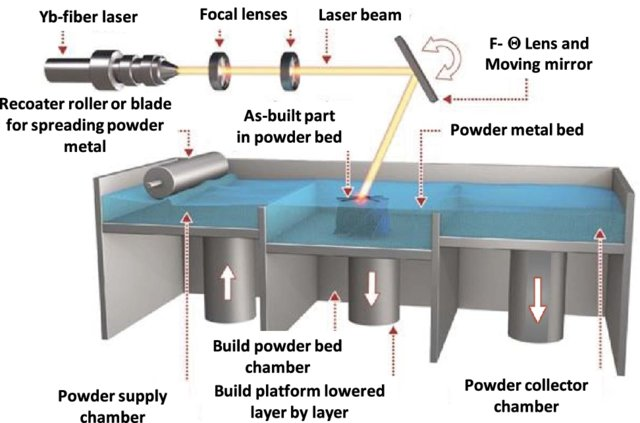
\includegraphics[scale=1.2]{Images/PBF.jpg}
    \caption[Laser PBF in AM.]{Laser powder bed fusion process in additive manufacturing. Adapted from \cite{ozel_focus_2020}.}
    \label{fig:PBF}
\end{figure}
Now, we will discuss the SLS printing process from start to finish. Firstly, the plate mounting is calibrated, and a vacuum atmosphere is created inside the printer chamber, or a regular flow of inert gas is introduced to obtain controlled and uniform melting of the metal powder to minimize oxidation and degradation of the powdered material. Directing an inert gas is preferred to maintaining a vacuum atmosphere in an industrial context mainly for two reasons. First, maintaining a vacuum atmosphere throughout the printing process requires much effort. Second, reducing the pressure in the process chamber can lower the metals' boiling point, leading to an excessive amount of smoke. The mixture of vaporized metal and smoke can affect the effectiveness of the laser. Indeed, a laser is an optical device and, as we all know, microparticles suspended in the air could deflect the laser beam. Once the inert gas flow is established, the roller or the blade responsible for distributing the powder performs a rapid powder re-coating. Then an electric resistor located under the powder bed preheats the powder at a temperature of about \SI{500}{\degreeCelsius}. This operation helps to reduce the gap between the temperature of the chamber and the metal's melting temperature and also helps maintain a uniform temperature within the build tray. This is necessary to prevent the warping of the part during the build due to non-uniform thermal expansion and contraction, which will lead to cracks and fractures (see Section \ref{sec:defects}). After these preliminary operations, the printing process can begin. A scanning system composed of a laser diode and a galvanometric mirrors system selectively melts the metal, alternating layer after layer with the powder distribution blade. LASER is an acronym that stands for "light amplification by stimulated emission of radiation," and it is a monochromatic beam of photons characterized by low divergence and a focal spot size of \numrange[range-phrase = --]{30}{80}\unit{\micro\metre}. Laser equipment can generate powers in the range of thousands of watts and can focus to beam spot sizes of fractions of a millimeter. These small spot sizes have the potential to create minuscule molten pools, reaching a velocity of up to several meters per second. Nowadays, almost all lasers used in AM rely on active optical fiber sources. A schematic representation can be seen in Fig. \ref{fig:detailedfiber}. 
\begin{figure}
    \centering
    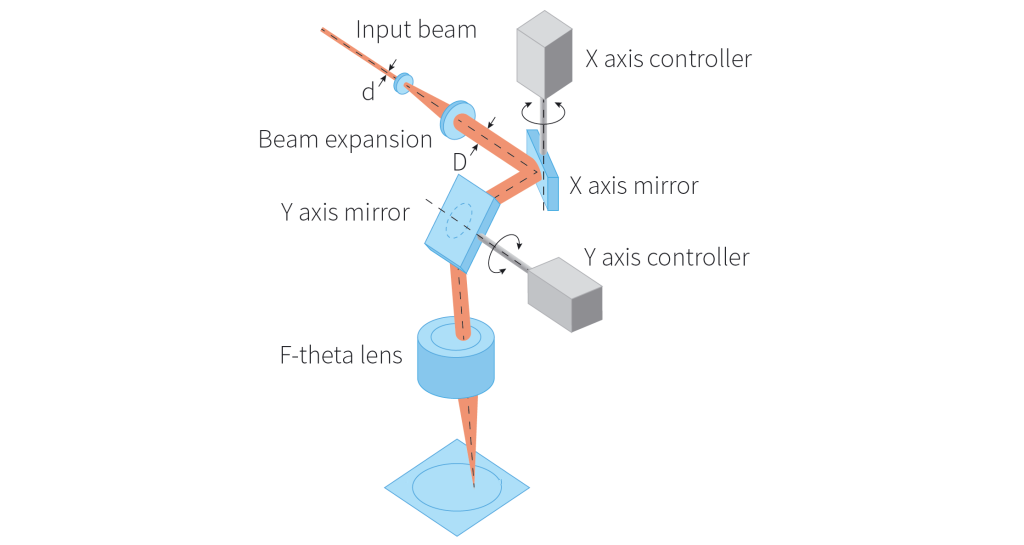
\includegraphics[scale=0.4]{Images/galvanometro.png}
    \caption[Galvanometric system.]{Dual-axis galvanometric system.}
    \label{fig:galvano}
\end{figure}
The energy transferred from the laser to the powder bed depends on the laser power (\numrange[range-phrase = --]{100}{1000}\unit{\watt}), the light-absorbing capacity of the material, and the scanning speed, which can be controlled (and it's limited) by the angular velocity of the galvanometer. The galvanometer system, Fig. \ref{fig:galvano}, consists primarily of two mirrors rotating along their axis, directing the laser beam to a desired point. The photon beam passes through a series of f-theta lenses that facilitate rapid laser movement and precise focusing of the laser spot. After completing the printing process, it is necessary to allow the object to cool down. Although supports are not always required, as the powder supports the object itself, they may need to be inserted to ensure uniform heat transmission during the printing and cooling phase. Once the object has cooled down, we can remove any excess powder. The excess powder can be recycled and reused after undergoing some preliminary processing and conformity controls \cite{strondl_characterization_2015}. Finally, post-processing operations can be carried out if required, such as removing any supports, surface finishing, and annealing. The latter is needed if the cooling phase inside the chamber has created an undesired microstructure in the printed piece.
% <<<SLS

%%%%%
%%%%%

% EBM >>>
\subsection{Electron Beam Melting}
\label{subsec:ebm}
In EBM printers, the process is fundamentally the same as in laser printers, with metal powder selectively fused in a powder bed, with a recoater blade to provide additional metal powder layer after layer. However, the energy source is not a laser (i.e., a beam of photons) but rather a beam of electrons. Secondly, the preheating stage is not accomplished through an electric resistor but through the electron beam. The preheating operation is one of the most significant differences between EBM and SLS. An electric current is passed through a metallic filament to produce an \emph{electron beam}, typically tungsten or tantalum. The resulting electron beam is then directed through a Wehnelt cylinder. By negatively or positively charging the cylinder, we can block or allow the passage of electrons respectively.
\begin{figure}
    \centering
    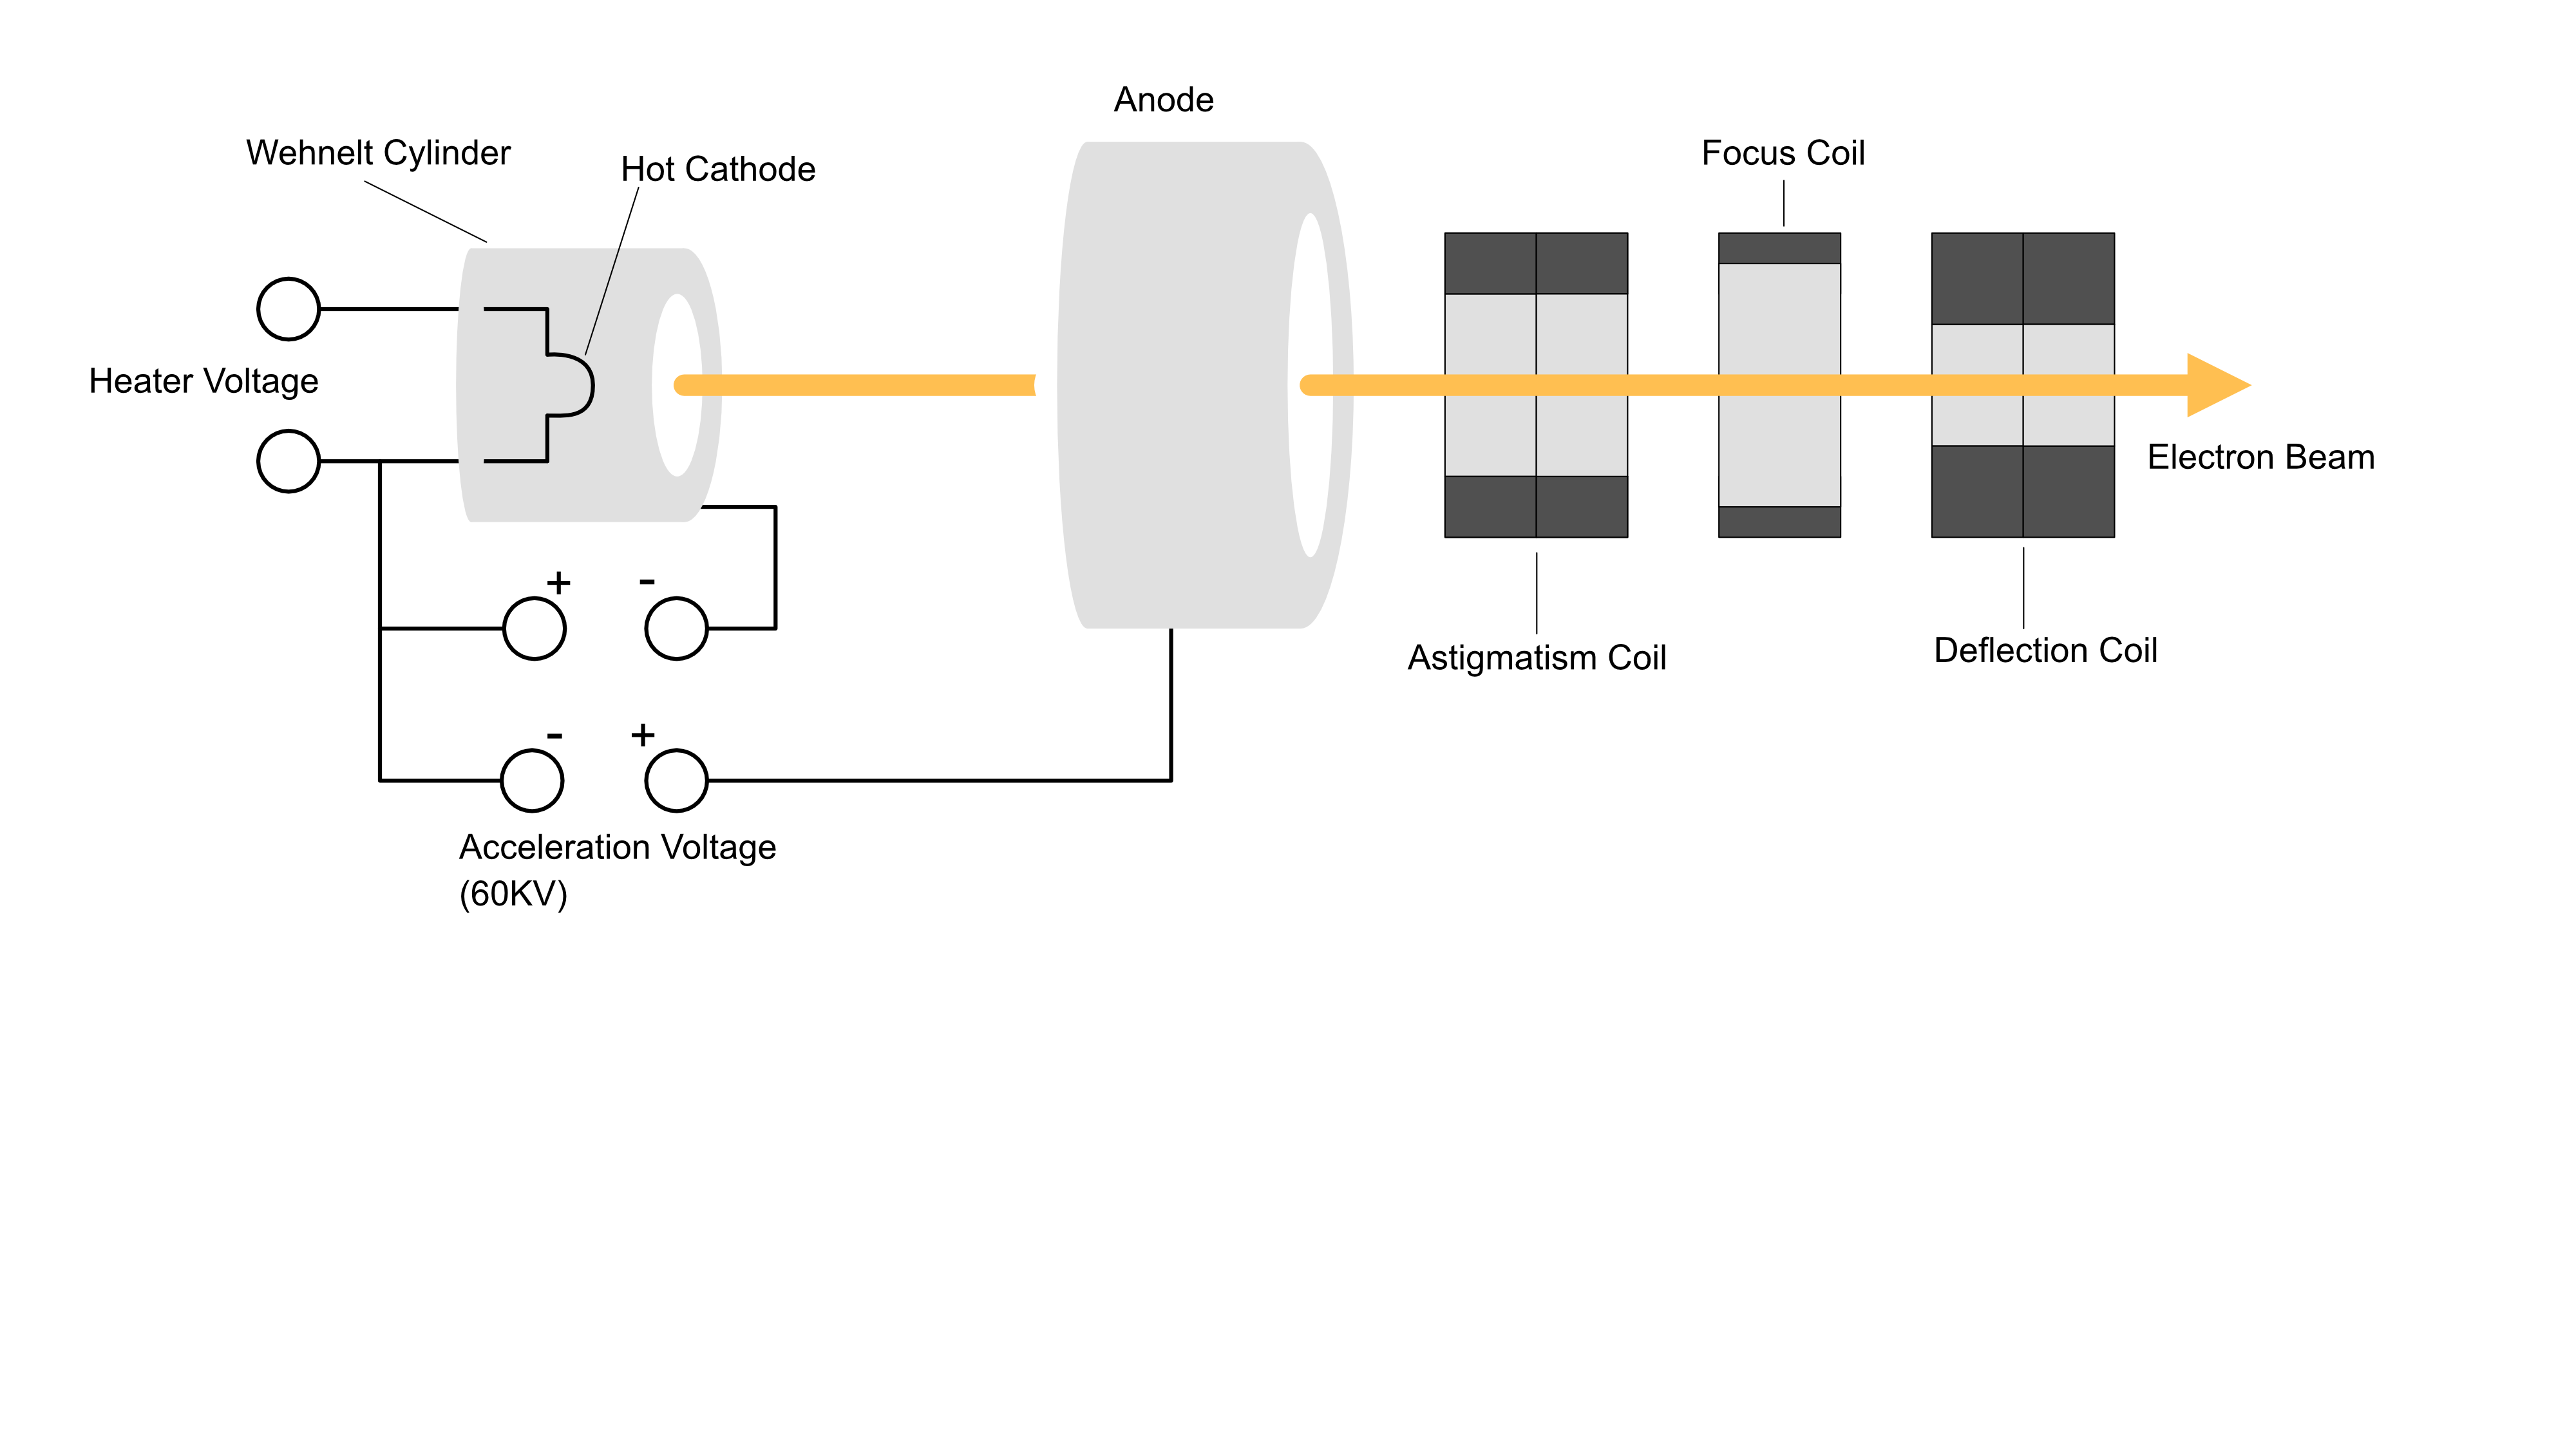
\includegraphics[width=0.75\textwidth]{Images/EBM.png}
    \caption[Electron gun schema.]{Electron gun schema.}
    \label{fig:electrongun}
\end{figure}
A diagram of the electron gun beam's structure can be seen in Fig. \ref{fig:electrongun}. Finally, the electron beam passes through an anode charged with a voltage of up to \SI{60}{\kilo\volt}, which accelerates the electrons and allows the beam to be directed into the column through magnetic lenses. Unlike SLS printers which rely on optical lenses, the lenses in EBM printers are magnetic lenses. A more comprehensive description of how magnetic lenses function will be provided in Section \ref{sssec:magneticlens}. EBM printers require a vacuum atmosphere inside the printing chamber to work correctly, and a minute amount of helium must be continuously injected into the chamber to prevent the accumulation of electric charges due to any residual electrons on the powder bed. The phenomenon will be discussed in Section \ref{subsec:ebminter}. To put the "minuscule amount" of helium required into perspective, consider that the pressure in the vacuum atmosphere inside the chamber is \SI{0.05}{\pascal}, and the pressure with helium flow is about \SI{0,2}{\pascal} (recall atmospheric pressure is \SI{1,01325e5}{\pascal}). The second significant difference, as mentioned earlier, is that the preheating phase does not occur through an electric resistor but rather through an initial scan of the electron beam that happens at two distinct moments. During the first phase, the entire powder bed is scanned, and during the second phase, only sub-regions of the powder bed that will be printed are scanned. Preheating phases help avoid the so-called "smoke effect" caused mainly by the electrostatic repulsion in the powder. Furthermore, the preheating stage is necessary for obtaining final objects with better performance and reduces the need for support structures during printing. This allows for the use of the entire volume of the powder bed container when printing and even printing multiple objects, one on top of the other, since there would be no printing supports interfering with them. This dual preheating phase causes the excess powder to solidify around printed pieces. Another structural difference of an EBM printer can bee seen in Fig. ~\ref{fig:ebm_printer}. Due to the vacuum inside the print chamber and the consequent lowering of the metal's vaporization temperature, a heat shield is required around the chamber to prevent the vaporized metal from condensing and creating a film on the entire printer structure. The heat shield acts as a physical barrier, allowing easy removal and disposal of the metal film produced during printing.
\begin{figure}
    \centering
    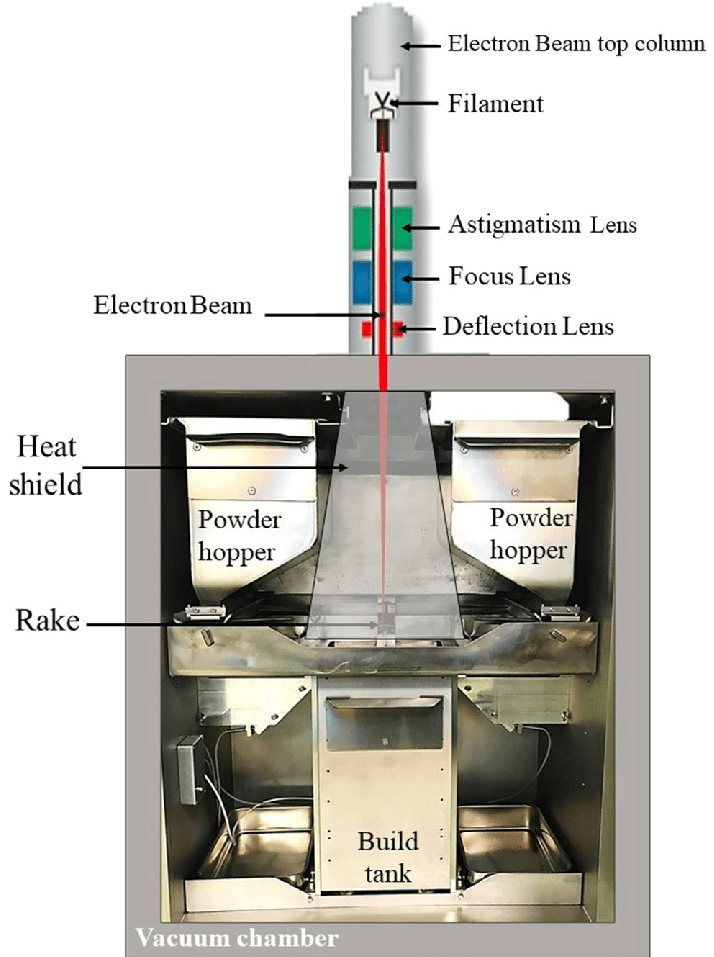
\includegraphics[scale=0.3]{Images/A-schematic-of-electron-beam-melting-EBM.png}
    \caption[EBM 3d-printer.]{Electron beam melting 3d-printer \cite{azam_-depth_2018}.}
    \label{fig:ebm_printer}
\end{figure}
\begin{table}
\small
    \centering 
    \begin{tabular}{|l l l|}
    \hline
    \rowcolor{bluepoli!40} % comment this line to remove the color
     & \textbf{EBM} & \textbf{SLS} \T\B \\
    \hline \hline
    \textbf{Energy source} & Electron beam & Laser  \T\B \\ 
    \textbf{Chamber atmosphere} & Vacuum(Almost) & Inert gas  \T\B\\
    \textbf{Scanning} & Magnetic lenses & Galvanometers \T\B \\
    \textbf{Energy absorption} & Conductivity-limited & Absorptivity-limited \T\B\\
    \textbf{Scan speeds} & Very fast & Limited by galvanometer inertia \T\B\\
    \textbf{Energy costs} & Moderate & High \T\B\\
    \textbf{Feature resolution} & \numrange{100}{200}\unit{\micro\metre} & \numrange{75}{100}\unit{\micro\metre}  \T\B\\
    \textbf{Materials} & Conductors & Polymers, metals and ceramic \T\B\\
    \textbf{Layer Thickness} & \SI{50}{\micro\metre} & \SIrange{10}{50}{\micro\metre}  \T\B\\
    \textbf{Min Wall Thickness} & \SI{0.6}{\milli\metre} & \SI{0.2}{\milli\metre} \T\B\\
    \textbf{Accuracy} & $\pm$\SI{0.4}{\milli\metre} & $\pm$\SI{0.3}{\milli\metre} \T\B\\
    \textbf{Build rate} & \numrange[range-phrase=--]{55}{80}\unit{\centi\metre^3 / \hour} & \numrange[range-phrase=--]{60}{100}\unit{\centi\metre^3 / \hour} \T\B\\
    \textbf{Powder Particle Size} & \numrange[range-phrase = --]{40}{105}\unit{\micro\meter} & \numrange[range-phrase = --]{15}{45}\unit{\micro\meter} \T\B\\
    \hline
    \end{tabular}
    \\[10pt]
    \caption{Comparison between SLS and EBM processes. Adapted from \cite{gallina_electron_2017}.}
    \label{table:slsvsebm}
\end{table}
There are also differences in the materials used for printing. In EBM printing, usually metal powder size is slightly larger than the powder used in laser printing, with a particle size of approximately \numrange[range-phrase = --]{40}{105}\unit{\micro\meter} against the \numrange[range-phrase = --]{15}{45}\unit{\micro\meter} in SLS processes. Furthermore, the metal powder must exhibit good electrical conductivity. Indeed, in EBM highly reflective metals can be used too because, unlike photons, electrons are not repelled by mirrored surfaces since they penetrate the matter thanks to the material's electrical conductivity.

To sum up what has been discussed so far, Table ~\ref{table:slsvsebm} highlights the main differences between the two processes described in previous sections.
% <<< End of EBM
% <<< End of Powder Bed Fusion Processes

%%%%%
%%%%%

% Metal Powders >>>
\section{Metal Powders for AM} 
\label{sec:metalpowders}
As we have seen in the section \ref{sec:pbf_proc}, PBF processes require metal powders. Various metallic materials can be transformed into powders suitable for additive manufacturing processes and applied in different sectors according to their mechanical properties. Table \ref{table:materialAMmetal} shows some examples of metallic materials currently available on the market and the respective industrial sectors in which they are used. In most cases, these powders are produced using atomization processes that exploit various physical methods to generate micro-particles, characterized by a more or less spherical shape and of which chemical purity depends on the method used. The inefficiency and cost of atomization processes used for manufacturing metal powders is why, in the case of specific high-quality powders, the powder price can be up to 10 times the cost of raw metal. \citeauthor{deng_origin_2020} (2020) have demonstrated that powders made of irregular micro-particles and with low chemical purity can lead to structural defects in the final parts, resulting in lower performance. Therefore, over the years, increasingly complex and expensive processes have been developed to obtain higher-quality powders.
\begin{table}[H]
\centering 
\small
    \begin{tabular}{|l l l|}
    \hline
    \rowcolor{bluepoli!40}
    \textbf{Material} & \textbf{Examples} & \textbf{Applications}\\
    \hline \hline
    \textbf{Stainless steel} & 316L, 174-PH, MS1, M300 & Food, biomedical, consumer \T\B\\
    \textbf{Ni-alloys} & In625, In718, In939 & Energy, motorsport\T\B\\
    \textbf{Al-alloys} & AlSi12, AlSi10Mg & Lightweight, aerospace, aviation\T\B\\
    \textbf{CoCr-alloys} & CoCrMo & Dental, biomedical\T\B\\
    \textbf{Ti-alloys} & Ti6Al4V, CP Ti & Biomedical, lightweight, aerospace\T\B\\
    \textbf{Tool steel} & Maraging 18Ni300 & Tooling, aerospace, automotive\T\B\\
    \textbf{Cu-alloys} & Bronze & Energy, heat exchanger\T\B\\
    \textbf{Precious} & Au, Pt, Ag & Jewellery, design\T\B\\
    \hline
    \end{tabular}
    \\[10pt]
    \caption{Material availability for metal AM.}
    \label{table:materialAMmetal}
\end{table}
\begin{figure}
    \centering
    \subfloat[\label{fig:wateratom}]{
        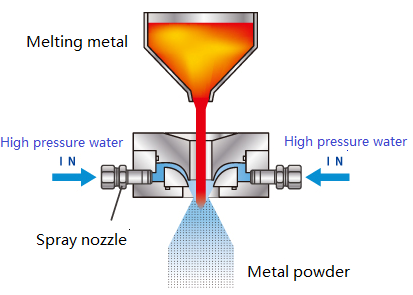
\includegraphics[scale=0.45]{Images/wateratom.png}
    }
    \qquad
    \subfloat[\label{fig:gasatom}]{
        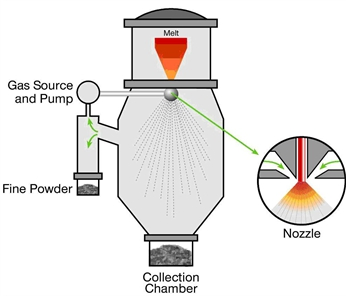
\includegraphics[scale=0.45]{Images/gasatom.png}
    }
    \\
     \subfloat[\label{fig:plasmaatom}]{
        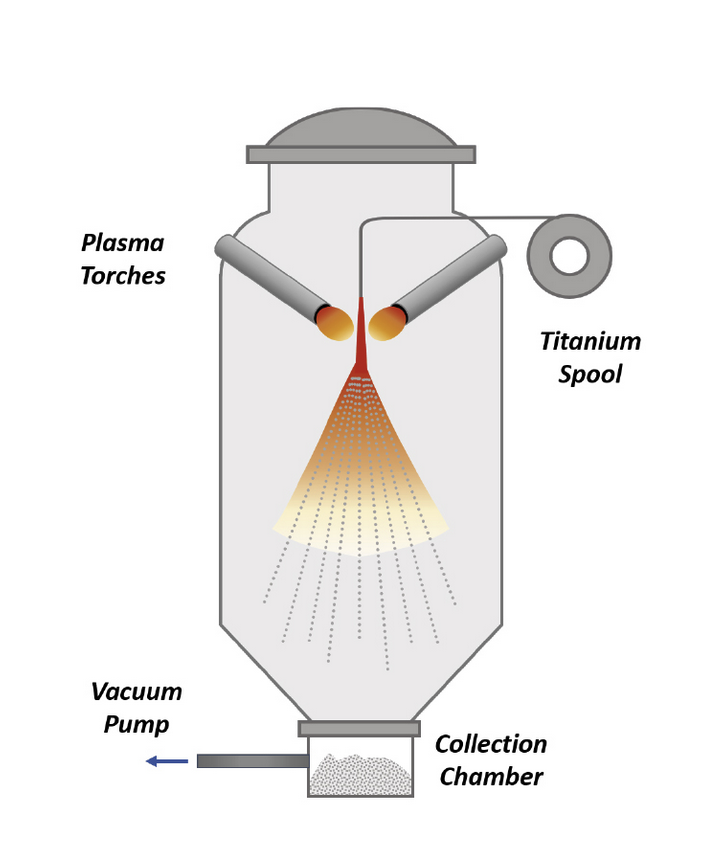
\includegraphics[scale=0.28]{Images/plasma.png}
    }
    \qquad
    \subfloat[\label{fig:repatom}]{
        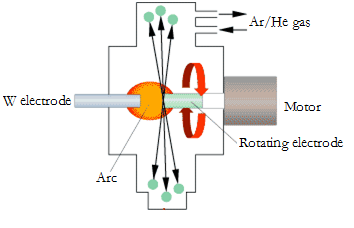
\includegraphics[scale=0.53]{Images/repatom.png}
    }
    \caption[Atomization processes.]{Water atomization process (a), gas atomization process (b), plasma atomization process (c), rotating electrode process (d) \cite{material_technology_innovations_co_rotating_2020, material_technology_innovations_co_water_2020, material_technology_innovations_co_gas_2020, inovar_communications_ltd_metal_2020}.}
    \label{fig:atom}
\end{figure}
\paragraph{Water atomization.}The process of water atomization of metals, Fig. \ref{fig:wateratom}, involves the production of small droplets of molten metal by exposing a stream of molten metal to a high-pressure jet of water. The water atomization process is typically carried out in a chamber where the molten metal is injected into a nozzle that directs the stream of liquid metal toward a high-pressure jet of water. As the molten metal comes into contact with the water, it rapidly cools and solidifies, forming tiny droplets collected at the bottom of the chamber. The size and shape of the metal droplets produced during the water atomization process can be controlled by adjusting the temperature of the molten metal, the pressure of the water jet, and the distance between the nozzle and the water jet. By handling these parameters, it is possible to produce metal powders with a range of particle sizes between \numrange[range-phrase = --]{1}{500} \unit{\micro\metre}. The output-to-input ratio for this process is approximately 95\%, which means that from \SI{1}{\kilo\gram} of raw metal, it is possible to obtain up to \SI{950}{\gram} of powder on average. Compared to other powder production methods, the water atomization process offers several advantages, including high production rates, the wide range of particle sizes obtainable, and the fact that metal ingots can be used as process input, shortening this production process's manufacturing chain. On the other hand, the process is characterized by a low chemical purity, irregular shape as can be seen in Fig. \ref{fig:waterpow}, and needs extensive post-processing operations to obtain a decent-quality product. Moreover, it cannot be used with reactive materials such as titanium and aluminum.
\paragraph{Gas atomization.} The process of gas atomization, Fig. \ref{fig:gasatom}, can be performed using a variety of gases, depending on processed metals. The most commonly used gases are inert gases such as nitrogen, argon, and helium, even if the latter is barely used in industrial applications due to its high cost. Inert gases are preferred because they do not react with the molten metal and do not introduce impurities into the metal powders. Metal ingots are molten, and the flow is rapidly solidified by exposing it to a high-pressure gas stream. This process's main advantages are its high production rate, wide range of obtainable particles, applicability to reactive materials, and ability to ensure good chemical purity. The main drawbacks are mostly related to the porosity of the resulting powder and the formation of small satellite particles.

\paragraph{Plasma atomization.} The process of plasma atomization, Fig. \ref{fig:wateratom}, involves the usage of high-temperature plasma torches to melt metal wire. We can generate a high-energy plasma by using an electric current through a non-consumable tungsten electrode and an inert gas jet to direct the welding arc into a focused area. As the molten metal droplets are expelled from the plasma jet, they rapidly solidify, sometimes also thanks to the water-cooled chamber, and break up into small, spherical powders, which are then collected in a container. The plasma atomization process offers several advantages over other powder production methods, including the ability to produce extremely spherical-shaped particles. Moreover, it can be used with reactive material. Plasma atomization can also produce powders with very high purity levels, as the high temperature of the plasma jet helps to eliminate impurities in the molten metal. However, it is more expensive than other powder production methods due to the need for specialized equipment and the high energy consumption required to generate the plasma arc. The process can also be challenging to control, as parameter variations can affect the resulting powders' size, shape, and purity. Powders produced using this method has a low size range of about \numrange[range-phrase = --]{1}{200}\unit{\micro\metre}.
\paragraph{Rotating electrode process.} In rotating electrode process, Fig. \ref{fig:repatom}, a consumable metal electrode is rotated at high speeds while an electric arc melts it in a chamber with a continuous inert gas flow. As the molten metal is exposed to the high-velocity inert gas stream, it rapidly solidifies and breaks into small droplets collected at the bottom of the atomization chamber. Due to its high cost, this production method is typically used when obtaining a metal powder with a perfectly spherical shape and without any impurities (gold, for example). If we take a look at Fig. \ref{fig:reppow}, we can easily grasp the potential of this technology in obtaining perfect spherical micro-particles.
\begin{figure}
    \centering
    \subfloat[\label{fig:waterpow}]{
        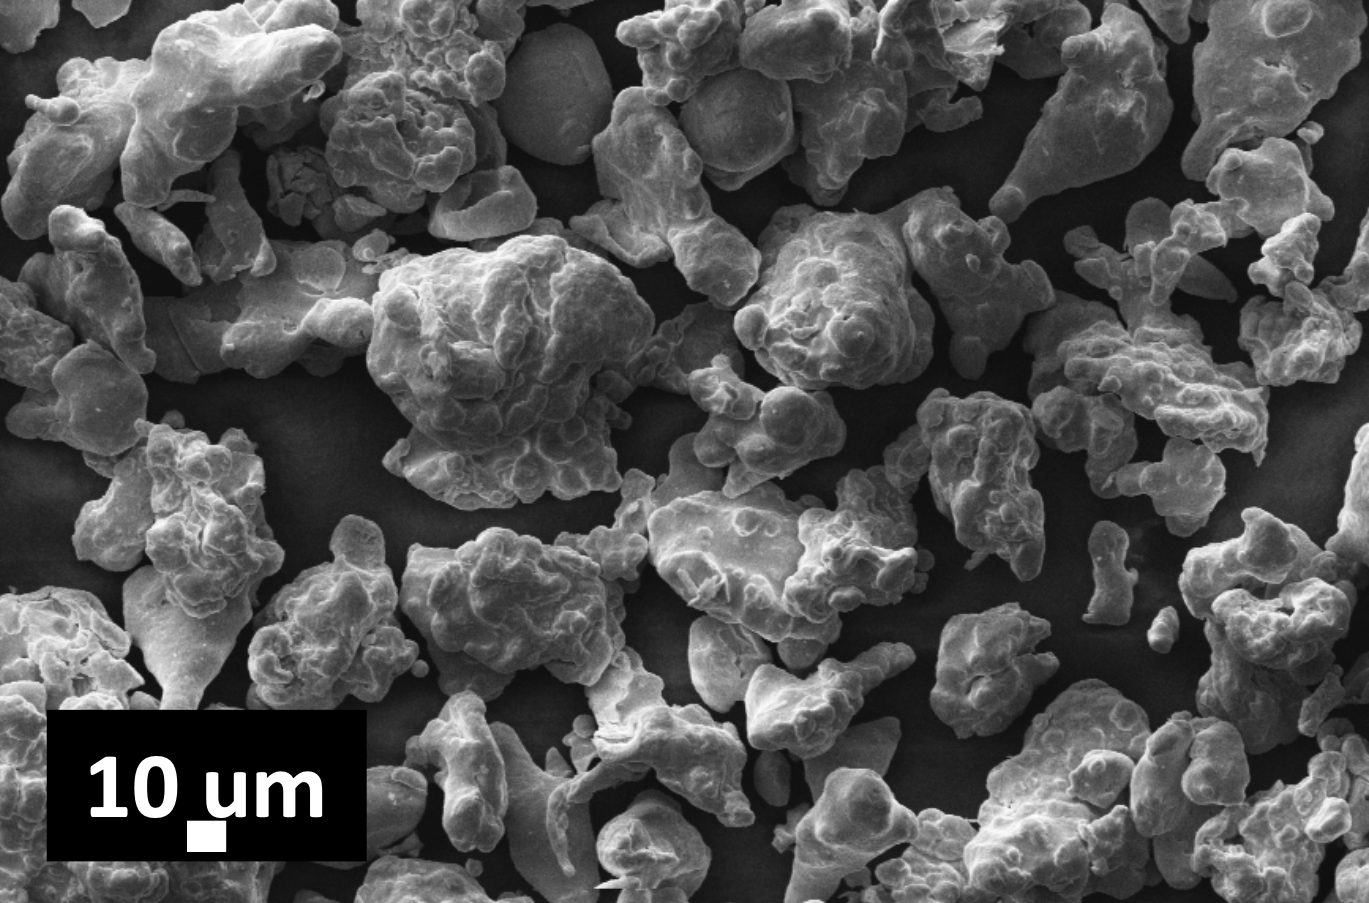
\includegraphics[scale=0.22]{Images/waterpow.png}
    }
    \qquad
    \subfloat[\label{fig:gaspow}]{
        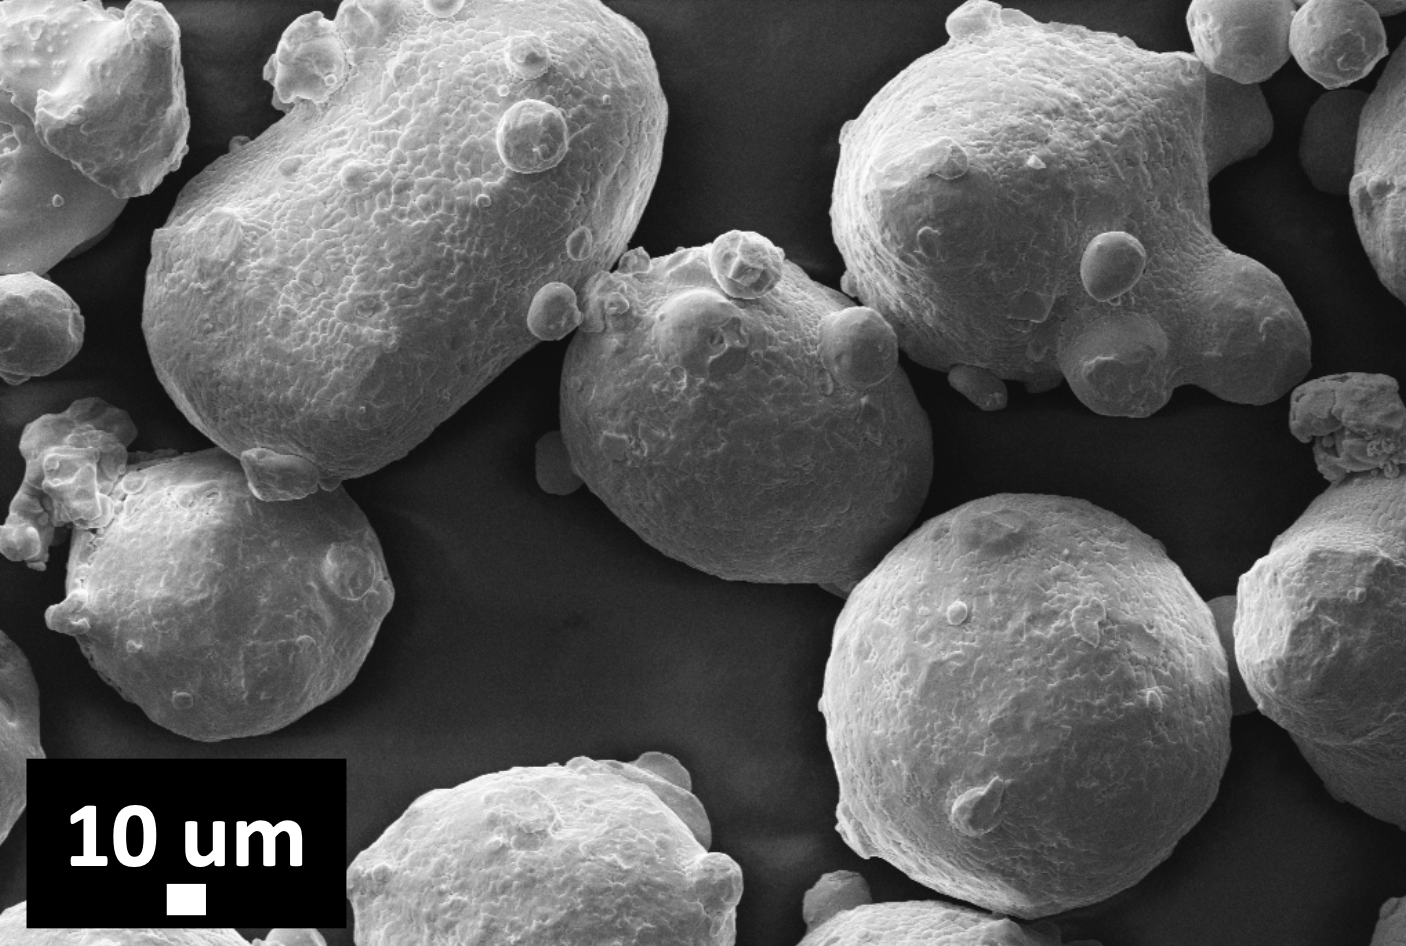
\includegraphics[scale=0.21]{Images/gaspowd.png}
    }
    \qquad
     \subfloat[\label{fig:plasmapow}]{
        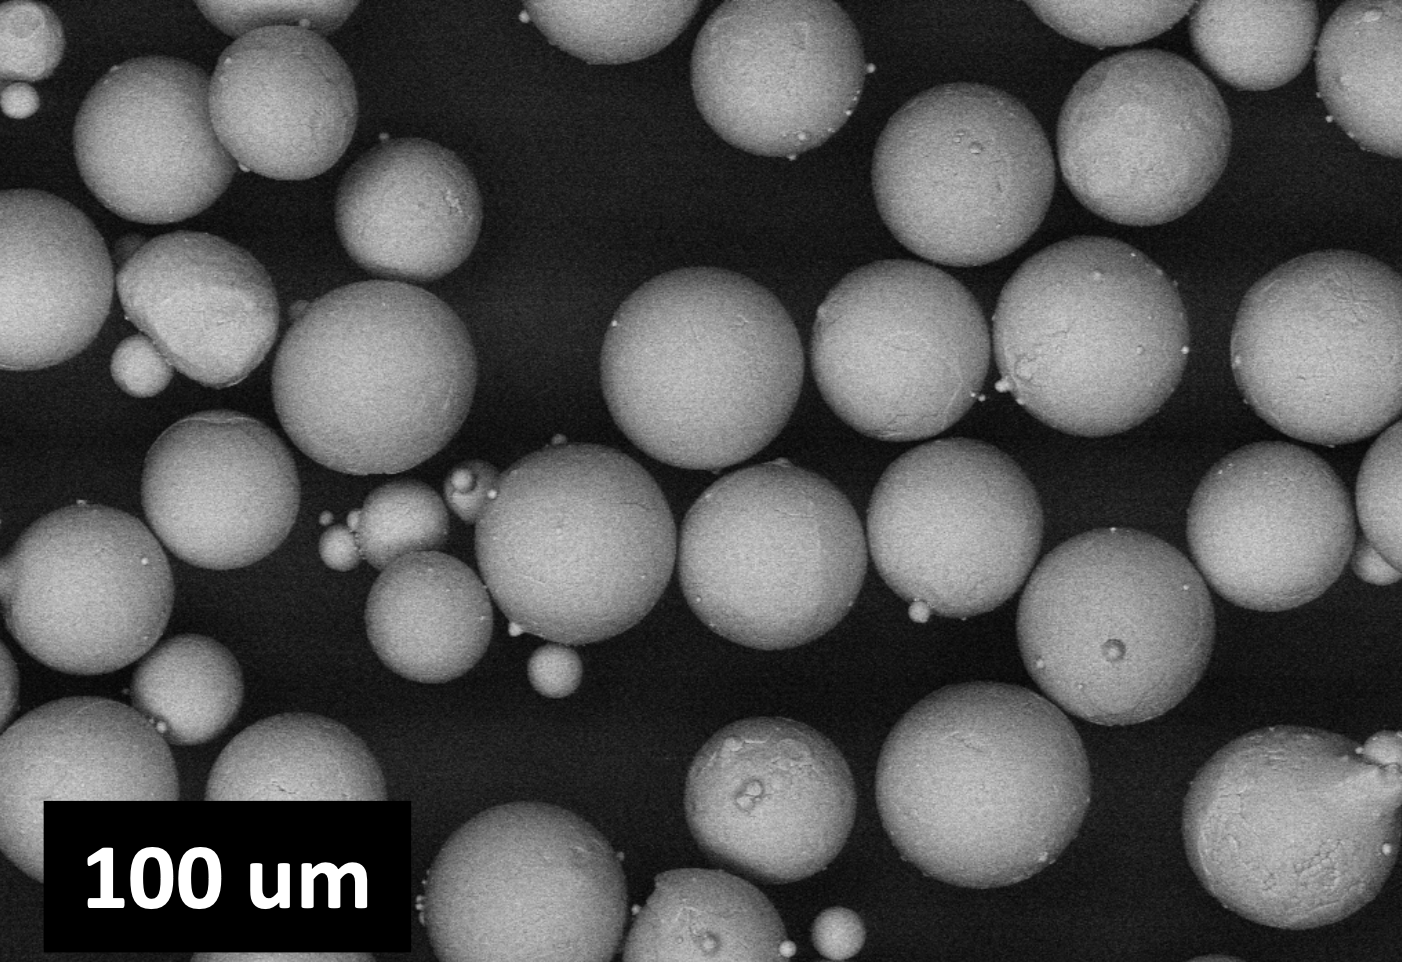
\includegraphics[scale=0.22]{Images/plasmapowder.png}
    }
    \qquad
    \subfloat[\label{fig:reppow}]{
        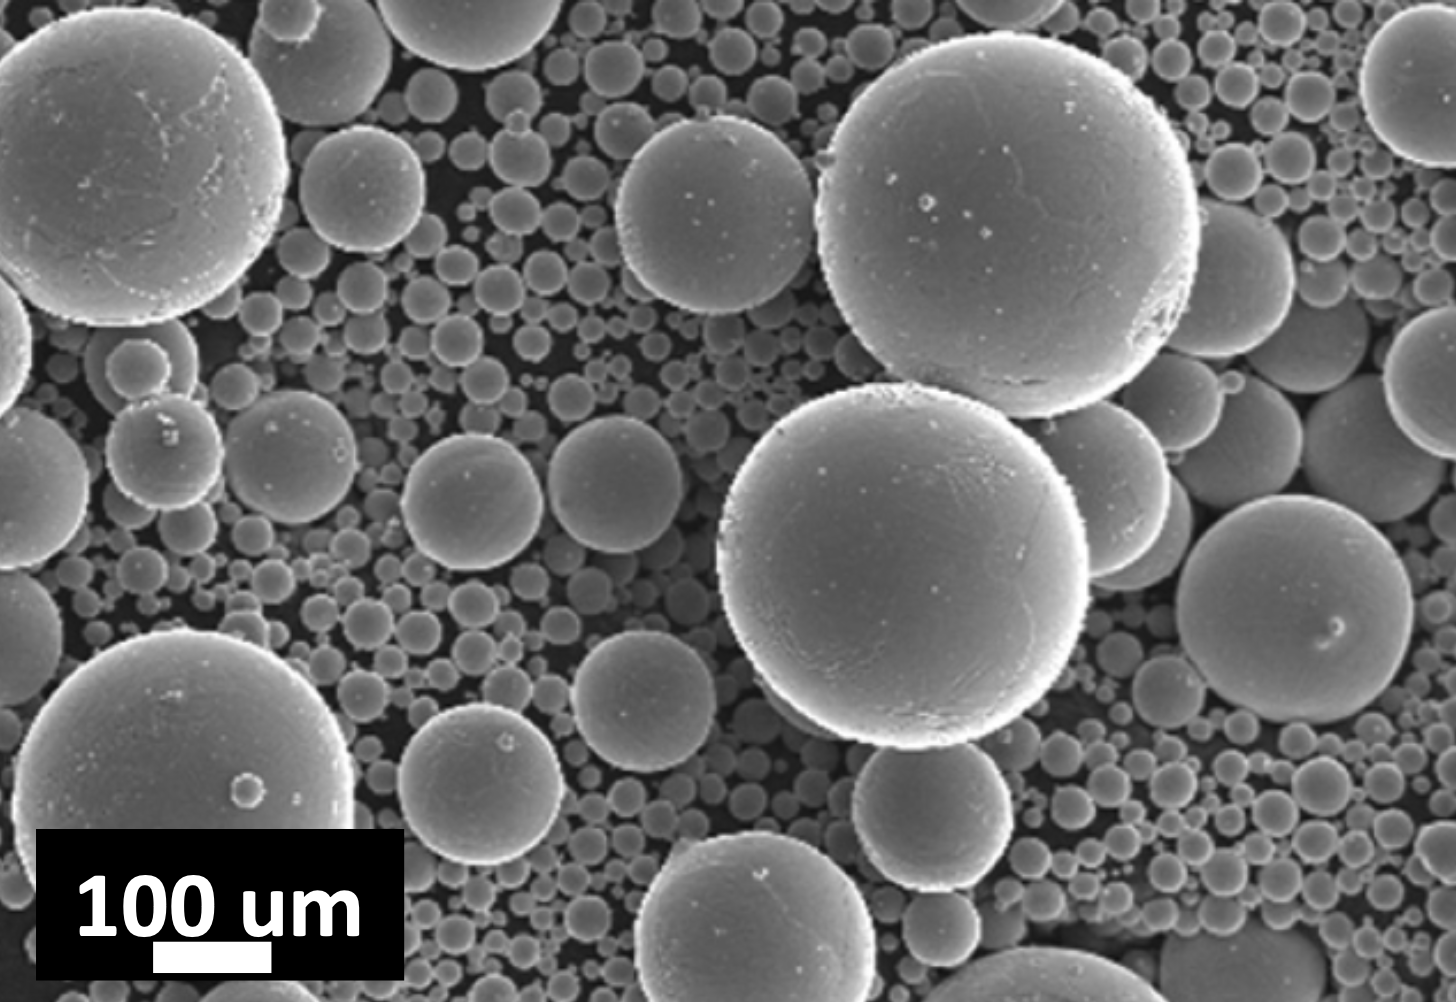
\includegraphics[scale=0.21]{Images/erppowder.png}
    }
    
    \caption[Powders from atomization processes]{Micro-particles obtained by water atomization (a), gas atomization (b), plasma atomization (c) and rotating electode process (d) \cite{slotwinski_characterization_2014}.}
    \label{fig:powders}
\end{figure}
% <<< End of Materials

%%%%%
%%%%%

% Energy matter interactions >>>
\section{Energy - Matter Interactions}
\label{sec:matterint}
This section should be regarded as "optional", and it's up to the reader's discretion whether to engage with it or not. In this section, we will delve deeply into the physical processes underlying the technologies discussed in Section \ref{sec:pbf_proc}. As said, in SLS, there is an interaction between a photon and metal powder, while in EBM, there is an interaction between electrons and metal powder. I will discuss first laser-metal interactions and then electrons-matter interaction.
\subsection{Laser - Matter Interaction}
\label{subsec:sintering}
The type and color of the laser are two essential features of SLS. Indeed, the energy transmitted to the material depends on the energy absorption characteristics of the material itself that vary according to the wavelength of the laser source. For the fusion process to be successful, metallic powder bed particles must receive enough energy to melt on the atomic level.
\begin{figure}
    \centering
    \subfloat[\label{fig:laserintera}]{
        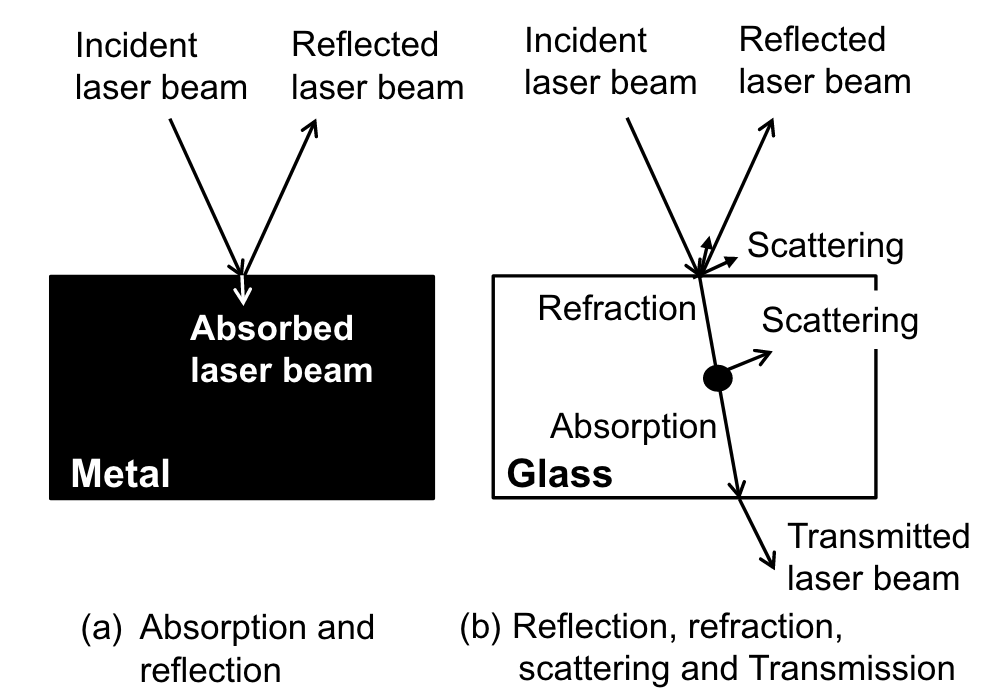
\includegraphics[scale=0.33]{Images/laser interactions.png}
    }
    \qquad
    \subfloat[\label{fig:laserintensity}]{
        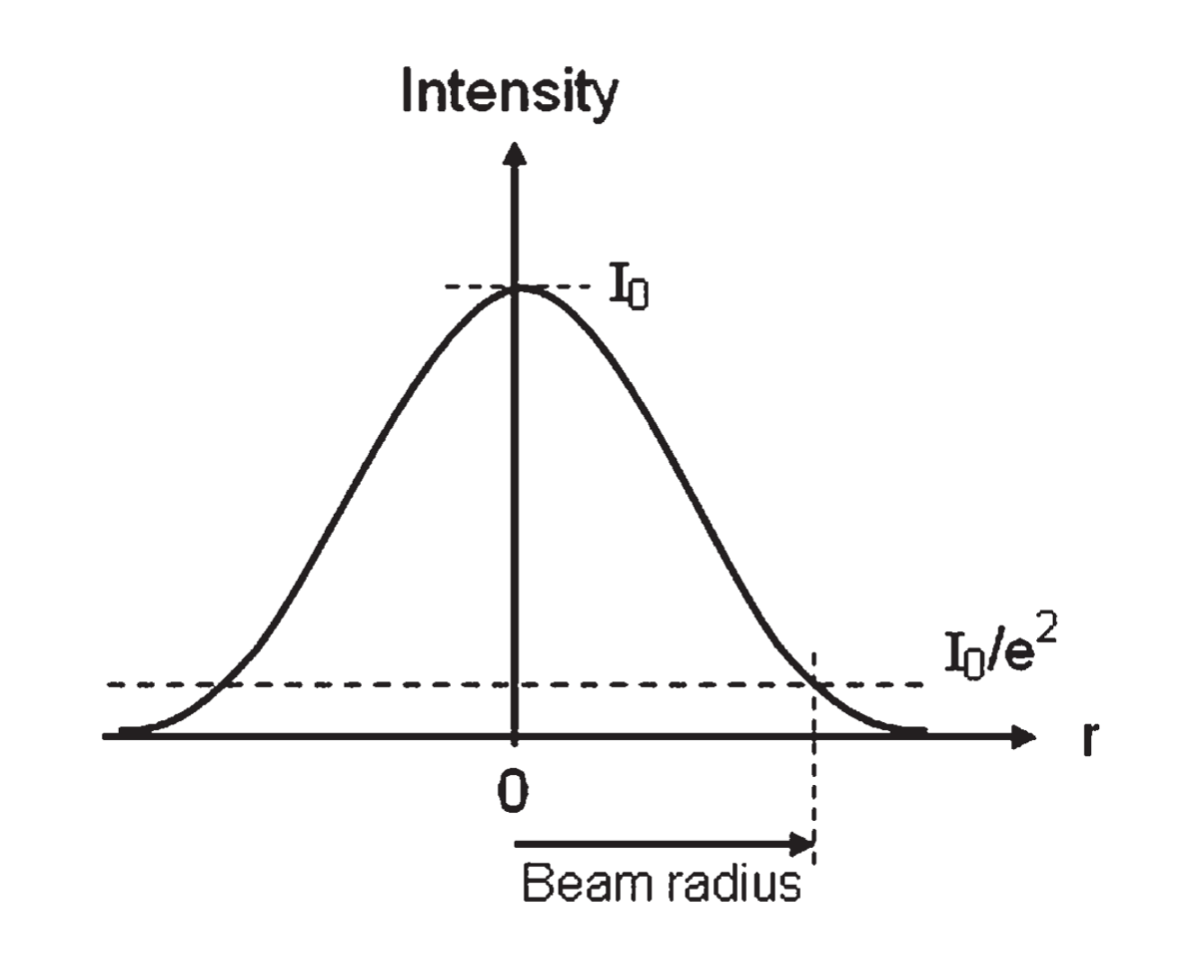
\includegraphics[scale=0.28]{Images/laserintensity.png}
    }
    
    \caption[Laser interactions and laser intensity.]{Schematic representation of physical interaction of absorption, reflection, transmission, refraction, and scattering between laser beam and material (a) \cite{katayama_fundamentals_2020}, and laser intensity schema (b).}
\end{figure}
For example, copper's absorptivity is about 50\% and 58\% for green and blue lasers, respectively. In other words, green and blue lasers are more advantageous in processing copper powder in terms of higher initial absorption than other laser typologies. As we will explore later, the electron beam transfers energy to the material through charge movement, while the laser beam operates as an optical device and hence it is more sensitive to the behaviors illustrated in Fig. \ref{fig:laserintera}. Indeed, the metal specimen is highly reflective and opaque. This is also the reason why the electron beam penetrates deeper into the metallic powder compared to the laser beam. The intensity of the laser emission varies as a function of the radius as 
\begin{equation}
    \label{eq:intensitylaser}
    I(r)=I_0\cdot e^{-2 \frac{r^2}{r_0^2}}
\end{equation}
and a schematic representation of density is shown in Fig. \ref{fig:laserintensity}.
The energy density of the laser beam is described by the equation
\begin{equation}
    \label{eq:energydensity}
    E_d = \frac{P}{h\cdot v \cdot d}
\end{equation}
where $E_d$ is the energy density (\unit{\joule/\milli\metre^3}), $P$ is the laser power (\unit{\watt}), $v$ is the laser scan speed (\unit{\milli\metre / \second}), $h$ is the hatch distance (\unit{\milli\metre}), $d$ is the layer thickness of the powder(\unit{\milli\metre}). For a more detailed description of heat transfer, please refer to the next section. The intensity of the laser beam's energy plays a crucial role in SLS because if it is not correctly calibrated, the final piece might exhibit porosities that compromise its mechanical features. Another critical parameter to consider during the SLS process is the duration of the laser pulse. As depicted in the Fig. \ref{fig:pulsipulsiocomepulsi} a prolonged laser pulse results in a broad heat zone, causing a shock wave that leads to an increased debris formation during the interaction that can interfere with new layers.
\begin{figure}
    \centering
    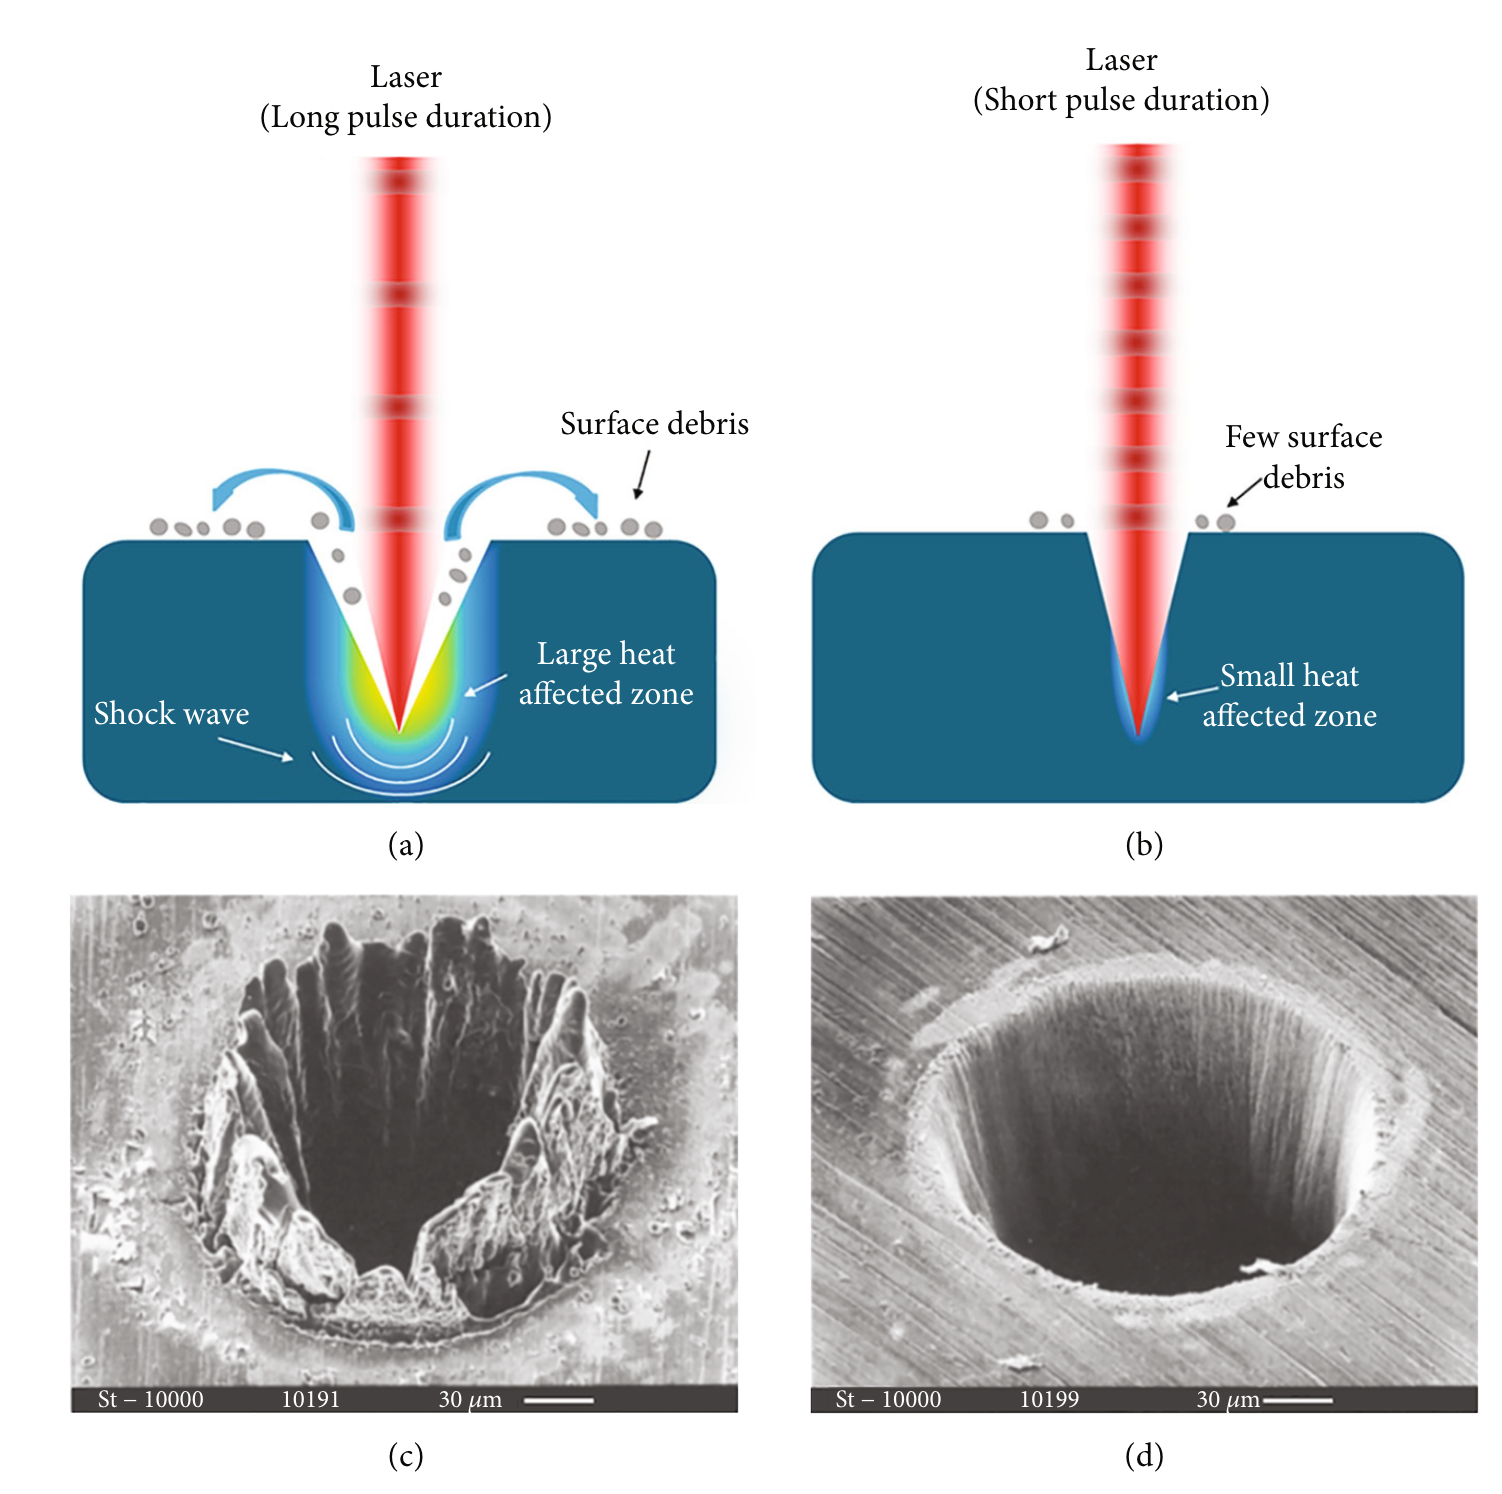
\includegraphics[scale=0.35]{Images/laserpulsing.png}
    \caption[Material absorptivity as function of wavelength.]{Schematic of laser interaction with materials under different pulse duration: (a) long pulse duration and (b) short pulse duration and respective holes fabricated on a steel foil by (c-d) \cite{lin_femtosecond_2021}.}
    \label{fig:pulsipulsiocomepulsi}
\end{figure}
For this reason, in recent years, there has been a shift towards using ultra-short pulse lasers. A schematic representation of one of this laser can be seen in Fig. \ref{fig:duripoco}. The laser in the figure is called "femtosecond laser" and is employed in manufacturing contexts such as precision processing or correction of semiconductors and liquid crystals, processing of transparent materials like glasses and sapphires, production of waveguide tubes for optical communication, drilling of engine components for cars and aircraft, among other applications \cite{katayama_fundamentals_2020}.
\begin{figure}
    \centering
    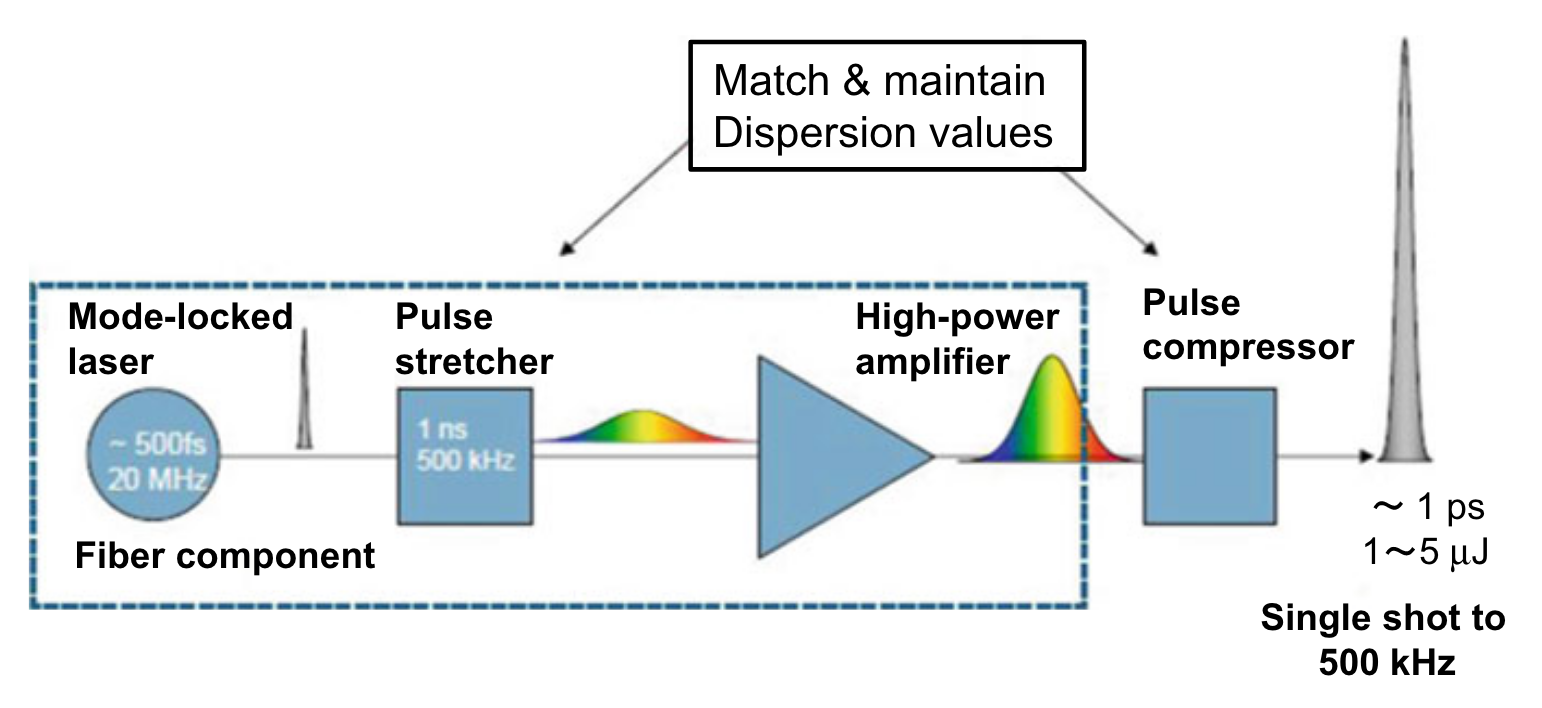
\includegraphics[scale=0.4]{Images/duripoco.png}
    \caption[Ultrashort pulse laser.]{Emission mechanism of ultrashort pulse laser \cite{katayama_fundamentals_2020}.}
    \label{fig:duripoco}
\end{figure}
\subsubsection{Heat transfer}
\label{sssec:heattransfer}
The heat and mass related events in SLS are influenced by both heat and mass movement. Laser heating is extremely rapid due to the fast scanning laser velocities. In a closed system, with respect to the first law of thermodynamics, the energy balance equation is formulated as follows \cite{bouabbou_understanding_2022}:
\begin{equation}
    \label{eq:tutteQ}
    Q_L = Q_C + Q_{CV} + Q_R,
\end{equation}
where $Q_L$, $Q_C$, $Q_{CV}$ and $Q_R$ respectively are the laser heat flux quantity, conduction, convection and radiation heat quantities. Recalling that only $Q_C$ will contribute to the melting process. Thus, some of the heat applied on the powder bed will be lost in the form of heat convection and radiation. \\
To describe the heat conduction, we can use Fourier's law:
\begin{equation}
    \label{eq:nonsiecapitouncazzo}
    \frac{\delta}{\delta x}\left(k \frac{\delta T}{\delta x}\right)+\frac{\delta}{\delta y}\left(k \frac{\delta T}{\delta y}\right)+\frac{\delta}{\delta z}\left(k \frac{\delta T}{\delta z}\right)+\dot{q} =\rho C_p \frac{\delta T}{\delta t}
\end{equation}
where $T$ (\unit{\kelvin}) is the temperature, $k$ (\unit{\watt.\metre^{-1}.\kelvin^{-1}}) is the thermal conductivity, $\dot{q}$ (\unit{\watt.\metre^{-3}}) is the rate of which the heat is applied to the system, $r$ (\unit{\kilo\gram.\metre^{-3}}) is the material density, $C_p$ (\unit{\joule. \kilo\gram^{-1}.\kelvin^{-1}}) is the specific heat and $t$ (\unit{\second}) is the interaction time between laser beam and powder particles.

\subsubsection{Optical Fiber Laser}
\label{sssec:fiberlaser}
One of the most common types of lasers used in SLS is the fiber optic laser \cite{milewski_additive_2017}. A diode is a semiconductor component acting like an unidirectional electric current gate. It permits current to pass effortlessly in one direction but significantly hinders its flow in the opposite one. Diodes have a polarity characterized by its anode (positive terminal) and cathode (negative terminal). Typically, diodes conduct current only when a positive voltage is supplied to the anode. In a laser diode (LD), an electric current is channeled directly through a dual hetero-junction structured semiconductor from the external side. When electrons recombine with positive holes at the active layer located between the n-type and p-type semiconductor zones, as shown in Fig. \ref{fig:np}, there is the emission of light beam.
\begin{figure}
    \centering
    \subfloat[\label{fig:np}]{
        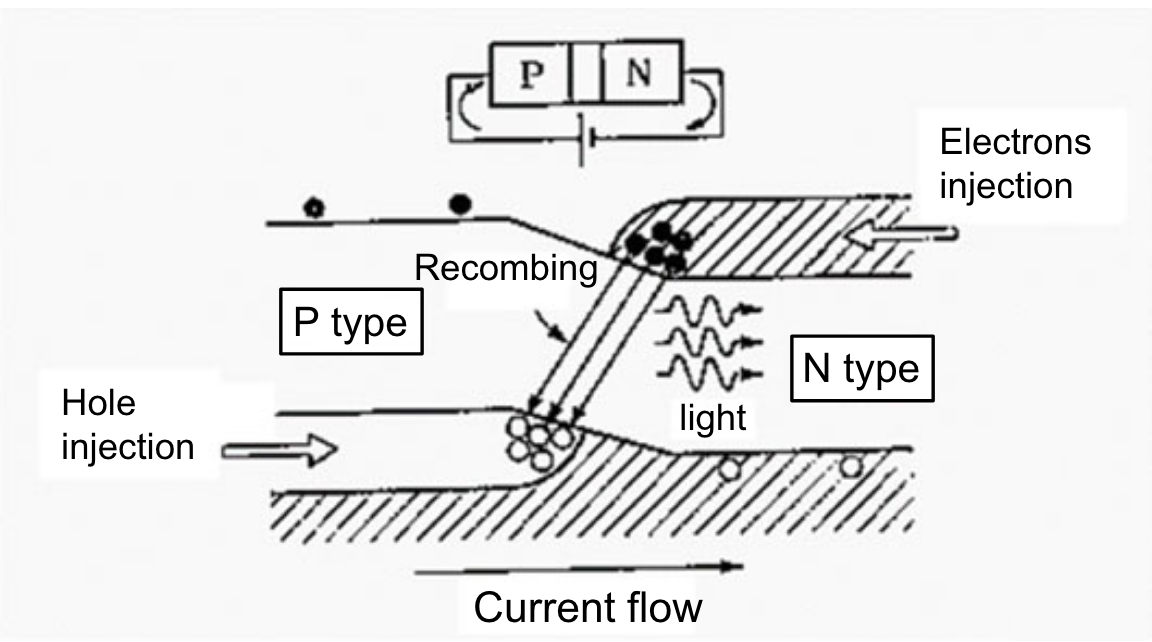
\includegraphics[scale=0.35]{Images/np.png}}
    \qquad
    \subfloat[\label{fig:detailedfiber}]{
        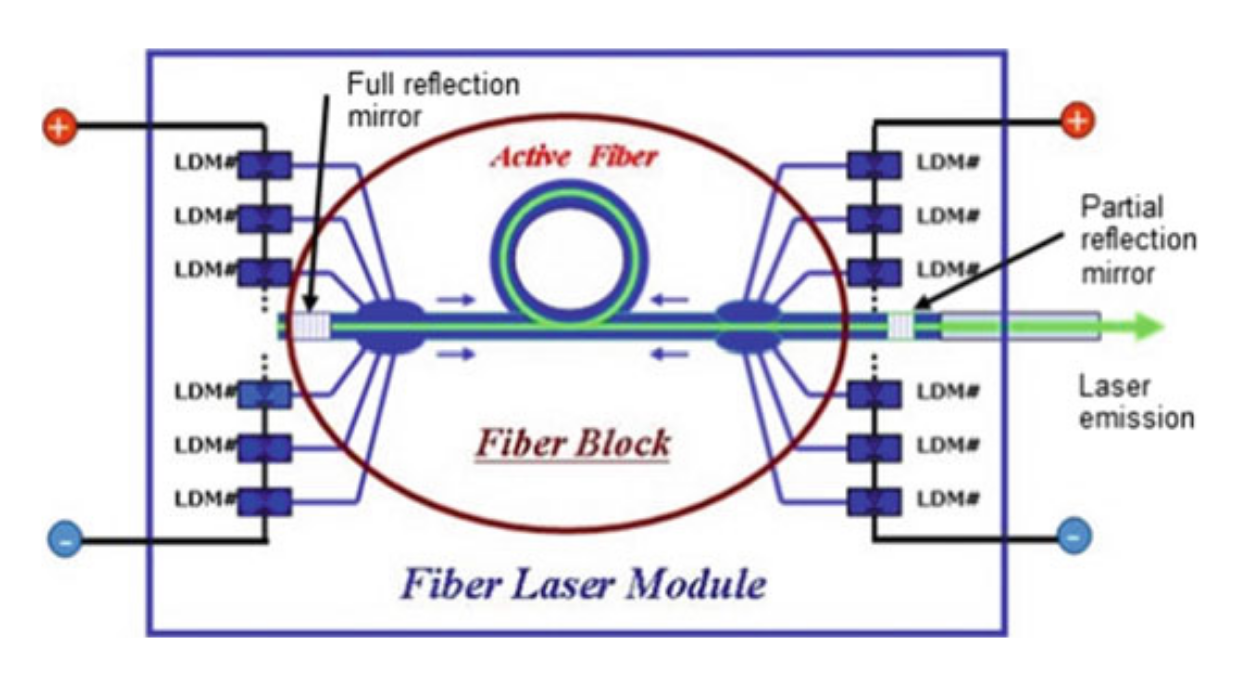
\includegraphics[scale=0.35]{Images/detailedfiber.png}}
    \caption[Laser diode and fiber laser.]{Emission mechanism of laser diode (a) and a detailed fiber laser schema (b) \cite{katayama_fundamentals_2020}.}
    
\end{figure}
In fiber lasers, the beam is emitted by an LD pumping and a fiber of high purity \ce{SiO2} quartz glass doped with \ce{Yb^3+} rare earth element. The diameter of the fiber is about \numrange[range-phrase=--]{10}{20}\unit{\micro\metre}. In this laser technology, optical pump diodes are coupled to an active laser fiber that has a unique reflective coating and Bragg gratings that reflect the laser light back and forth along the length of the fiber to create a coherent beam of light at the output of the laser \cite{milewski_additive_2017}. In Fig. \ref{fig:detailedfiber} we can see full reflection mirror and partial reflection mirror installed next to the fiber. This also means that the laser beam adjustment is not needed, which means easier handling of the system. Combining multiple laser modules using a beam combiner for a more powerful laser is also possible. We can use additional optical fibers to deliver and contain the light energy, providing a robust, flexible, and fully enclosed beam path for beam delivery \cite{milewski_additive_2017}. Fiber laser has many \textit{advantages} such as high beam quality, the fact they are small and lightweight, high intensity (which allows higher scan speed) and high efficiency (cost decreasing), long-distance delivery, and require basically no maintenance. 
\subsection{Electrons-Matter Interaction}
\label{subsec:ebminter}
According to \citeauthor{schultz_h_electron_1994} (1994), while the physical characterization of electron beams has been recognized since the 1960s, the microscopic processes are such that they remain without a comprehensive quantitative explanation also nowadays. However, a comprehensive explanation of electrons properties and their interaction with matter was given by \citeauthor{krumeich_properties_2015} (2015).
\subsubsection{What is an Electron?}
\label{sssec:electron}
An electron is a fundamental subatomic particle that carries a negative electric charge and is one of the primary constituents of atoms. As explained in Section \ref{subsec:ebm} the electron beam is made of electrons generated through the thermionic effect with a metallic filament, typically tungsten or tantalum. At the cathode, an accelerating voltage $V$ is applied, causing electrons acceleration till velocity $v$. As explained in \citeauthor{krumeich_properties_2015} (2015), we can write the equation for kinetic energy associated to an electron as 
\begin{equation}
    \label{eq:energyelectron}
    E  = e\cdot V = \frac{1}{2}mv^2
\end{equation}
Given the fact that electron mass is \SI{9.109e-31}{\kilo\gram}, electron charge is \SI{-1.602e-19}{\coulomb} and that a common voltage for EBM application is \SI{60}{\kilo\volt}, from \ref{eq:energyelectron} we find that electron velocity is
\begin{equation}
\label{eq:velocityelectron}
v=\frac{\sqrt{2\cdot e\cdot V}}{m}
\end{equation}
which is approximately \num{1.453e8} \unit{m/s} (about half the speed of light). Recalling the dualism wave-particle of the electron, we can use De Broglie equation to compute the wavelength of the electron beam \cite{krumeich_properties_2015}:
\begin{equation}
\label{eq:wavelength}
    \lambda = \frac{h}{\sqrt{2\cdot m \cdot e \cdot V}}
\end{equation}
where $h=$\SI{6.62607015e-34}{\joule.\second} is Planck constant. In case of a voltage higher than \SI{300}{\kilo\volt}, it's necessary to include a term that accounts for the relativistic nature of mass in \ref{eq:wavelength}, as the electron's speed would approach the speed of light.
\subsubsection{Magnetic Lenses in EBM}
\label{sssec:magneticlens}
In EBM, electromagnetic lenses control the beam emission. As the beam passes through these lenses, the astigmatic lenses adjust the shape of the electron beam spot, the focus coil changes the spot size, and the deflection coil moves the beam along the x and y axes.
\begin{figure}
    \centering
    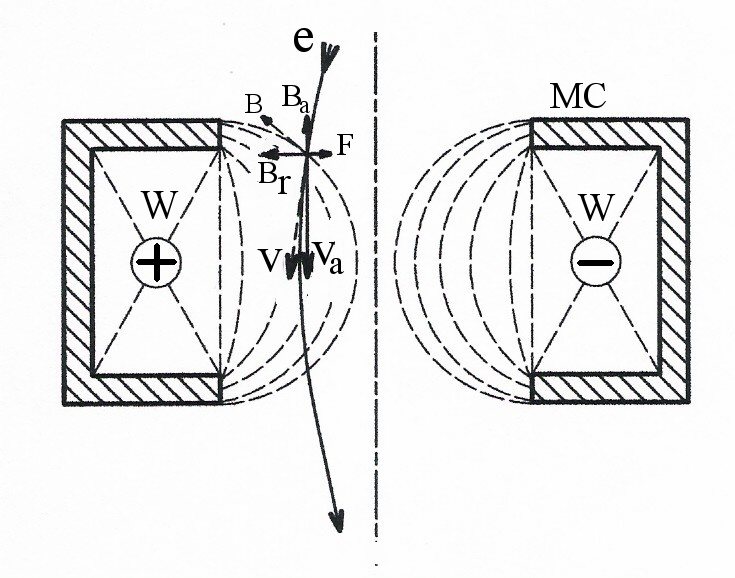
\includegraphics[scale=0.7]{Images/Magnetic_lens.jpg}
    \caption[Magnetic lens.]{Forces schema when an electron beam pass through magnetic lens \cite{wikipedia_magnetic_2023}.}
    \label{fig:magneticlens}
\end{figure}
The force $\mathbf{F}$ which an electron of charge $-e$ experiences when traveling with a velocity $\mathbf{v}$ due to a magnetic field $\mathbf{B}$ is given by Lorentz's law:
\begin{equation}
    \mathbf{F} = -e\cdot \left( \mathbf{v} \times \mathbf{B}\right)
\end{equation}
We can decompose the magnetic field into a radial component $\mathbf{B}_R$ and an axial component $\mathbf{B}_L$. The initial direction of the electron is parallel to the axis. Thus, it is subjected to the radial component $\mathbf{B}_R$ only, which is responsible for an orthogonal force to $\mathbf{v}$. Hence, electrons start rotating. When they start spinning, they are subject to the axial field of the magnetic field too, which results in a reducing radius spiraling trajectory that converges the beam towards the target.
\subsubsection{Electrons Interaction}
\label{sssec:electroninteractions}
\begin{figure}
    \centering
    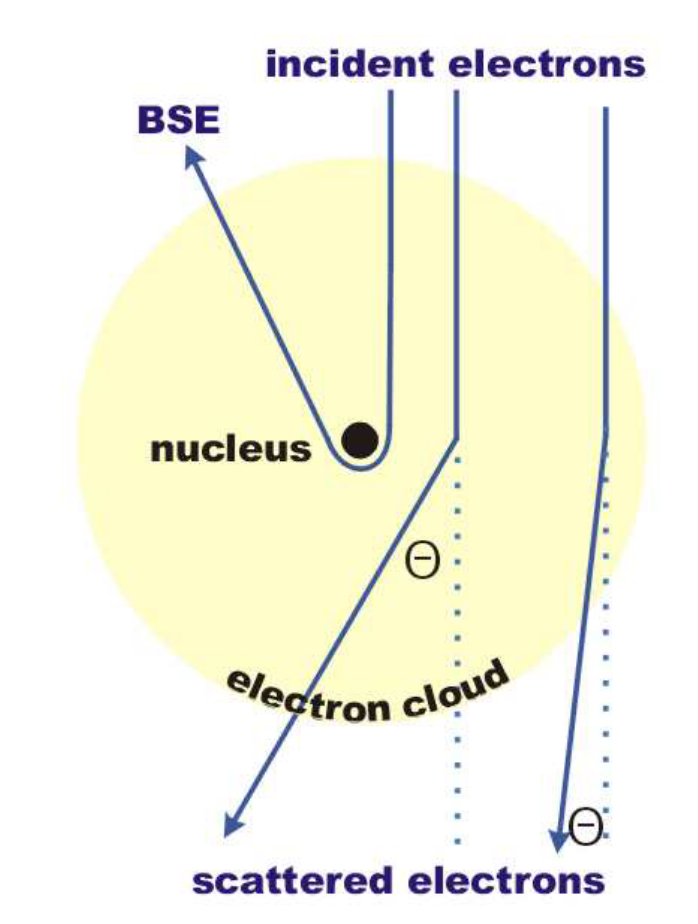
\includegraphics[scale=0.35]{Images/electrons.png}
    \caption[Scattering and backscattering of an electron.]{Scattering and backscattering effect of an incident electron inside the electron cloud of an atom \cite{krumeich_properties_2015}.}
    \label{fig:electronsscattering}
\end{figure}
As explained in \citeauthor{korner_additive_2016} (2016), we can distinguish two interaction types between electrons and matters, defined on the basis of transferred energy quantity. 
\paragraph{Elastic interactions} The electron's energy remains constant: when electrons delve into the surface, they engage as negatively charged entities with the metal's negative field and the positive charge from the nucleus's protons. Electrons can be rerouted on a different path without losing kinetic energy (known as elastic scattering). After several interactions, these deflected electrons might sometimes exit from the metal. This phenomenon is called backscattering. In Fig. \ref{fig:electronsscattering}, there is a representation of all the possible interactions between an electron and an atom nucleus. This event occurs because of the Coulomb interaction, which happens when a negatively charged entity (electron) comes close to a positively charged one (nucleus). Coulomb force is described by the equation:
\begin{equation}
    \label{eq:coulomb}
    F=\frac{Q_1\cdot Q_2}{4\pi \varepsilon_0 r^2}
\end{equation}
where $r$ is the distance between the charges $Q_1$ and $Q_2$ and $\varepsilon_0=$ \SI{8.854e-12}{\farad / \metre} is the dielectric constant. The backscatter phenomenon is determined by material characteristics and the angle at which the beam hits the metal surface. See Fig. \ref{fig:backscattering}. It represents an energy deduction from the melting procedure. Indeed, if an electron exits the material, it cannot transfer energy to the material itself. So, for process efficiency, we have to avoid these interactions. The backscattering effect is directly proportional to the atomic number $Z$ of the material of the powder, specifically $Z^2$.
\begin{figure}
    \centering
    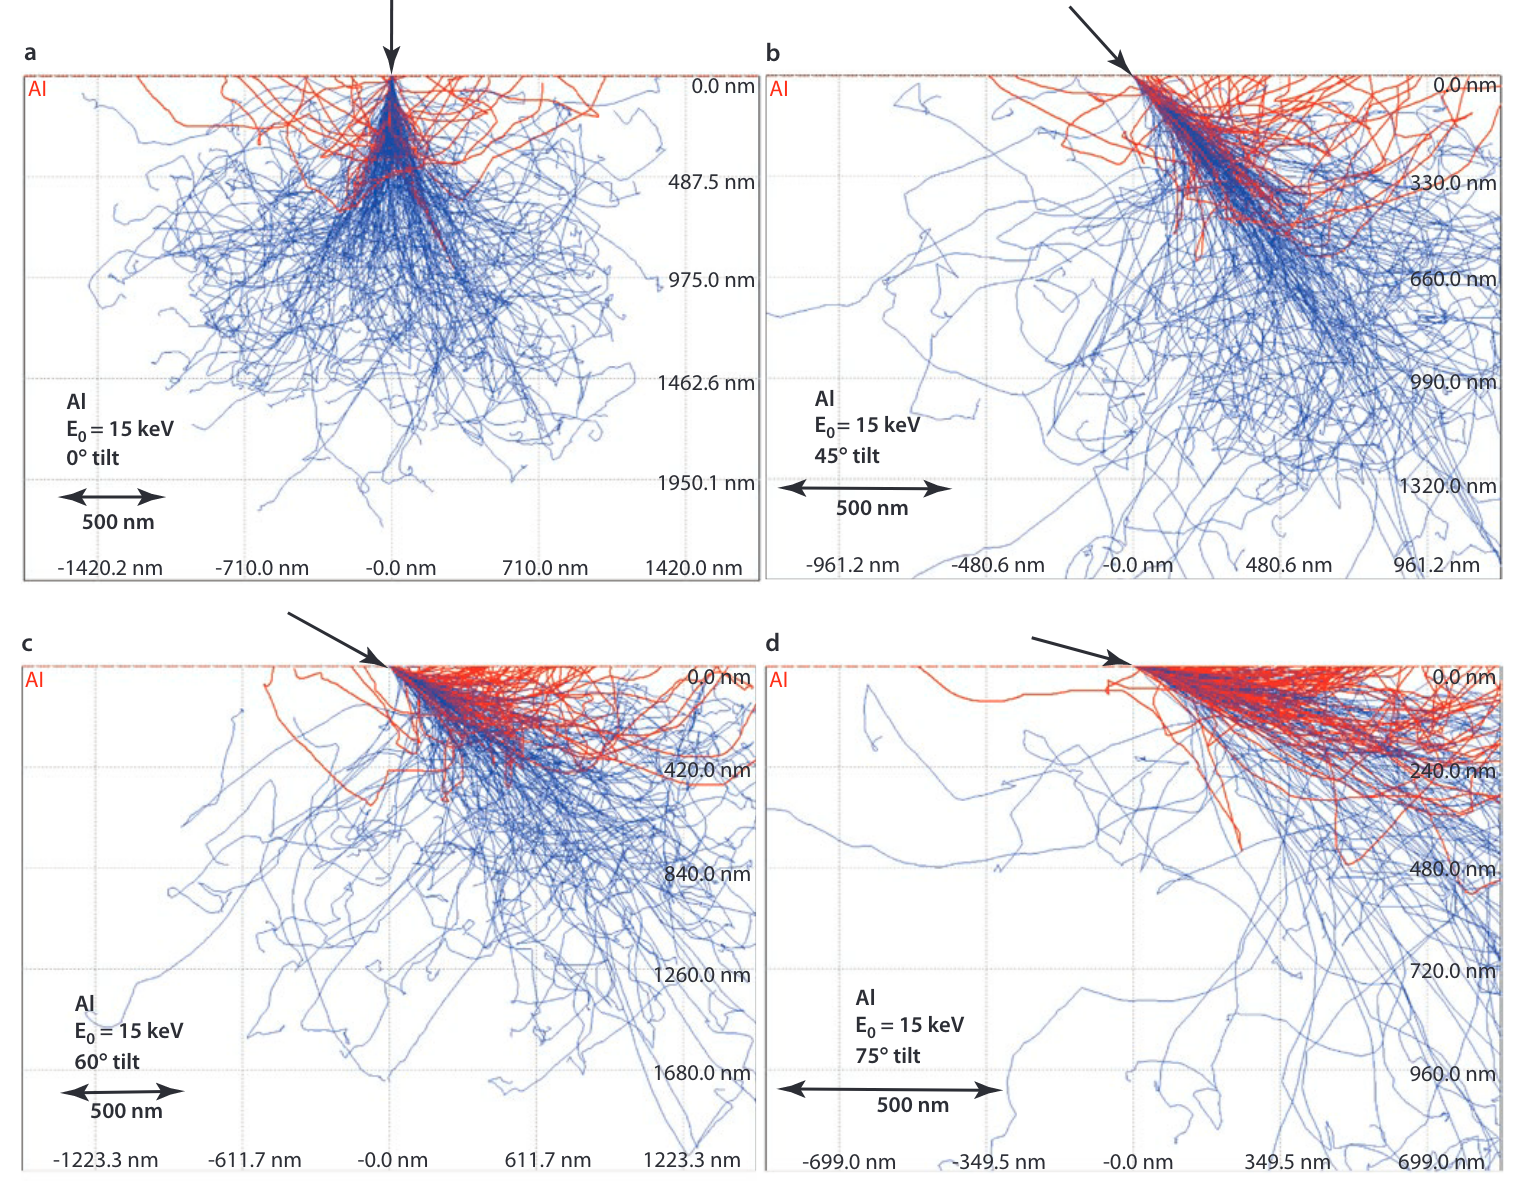
\includegraphics[scale=0.4]{Images/backscattering.png}
    \caption[Backscattering of an electron at different angles.]{Montecarlo simulation for an aluminum specimen hit by an electron beam at different angles, \ang{0}, \ang{45}, \ang{60}, \ang{75} respectively \cite{goldstein_scanning_2018}. In red, backscattered electrons.}
    \label{fig:backscattering}
\end{figure}
A fine and as spherical as possible powder is essential to reduce the backscattering effect caused by the incidence angle. In EBM processes, the more spherical the particles are, the more we can assume that the electron beam will strike the particle surface perpendicularly. We can see in Fig. \ref{fig:rotondette} why.
\paragraph{Inelastic Interactions:} In inelastic interactions, the energy of the electrons diminishes. The energy imparted to the sample results in the heating of the metal and its corresponding melting. These interactions cause the release of certain emissions, detailed below \cite{krumeich_properties_2015, goldstein_scanning_2018}:
\begin{itemize}
    \item \textbf{Inner-shell ionization :} The energy is passed to an inner electron, which is adequate to eject it from the atom. This results in an unstable atom configuration, leading to the release of X-rays or an Auger electron. \emph{X-rays} are produced when an inner electron is released into the vacuum, and an electron from the valence shell descends to occupy the void left by the electron from a deeper level. On the other hand, an \emph{Auger electron} is produced when the core electron, stimulated by the electron beam's energy, is expelled into the vacuum. Another electron from a higher level occupies the left space, which then radiates energy to a closer electron until it is released into the chamber. That's why, in an EBM 3D printer, it is crucial to have a shield to protect operators from X-rays.
    \item \textbf{Braking radiation:} The electron that enters the atom slows down due to its interaction with the positively charged nucleus. The subsequent reduction in energy is released as X-rays. The material completely absorbs X-rays of lower energy, while X-rays of higher energy are released in the printing chamber.
    \item \textbf{Secondary electron:} Electrons within the valence band require minimal energy to surpass the potential barrier, and various electron-matter interaction mechanisms can provide this energy. This can cause the release of these electrons in the printing chamber. The inert gas flow in the chamber removes these electrons from the powder bed since they can interfere with the printing process.
    \item \textbf{Cathodoluminescence:} when an electron from the valence band rises to the conduction band, a vacancy is created in the valence band. Another electron descending from the conduction band occupies this vacancy, which releases a photon. This phenomenon is responsible for the characteristic light produced when the electron beam hits the metal powder in EBM. 
    \item \textbf{Plasmon:} an electron moving through the collection of electrons in the valence band can cause a disturbance, leading to a collective vibration of the free electrons. This interaction is prevalent in metals but can also occur in any substance with free electrons. This phenomenon is responsible for the creation of plasma oscillation.
    \item \textbf{Phonons:} Phonons are understood as the collective oscillations of atoms within a crystal lattice, resulting from inelastic engagements with the electron beam. When an atom initiates this vibrational movement, it conveys this activity throughout the lattice, impacting a significant volume. Phonons are the only ones responsible for the melting of metal powders. Other products are undesirable or even accountable for side effects during the printing process.
\end{itemize}
\begin{figure}
    \centering
    \subfloat[\label{fig:rotondette}]{
        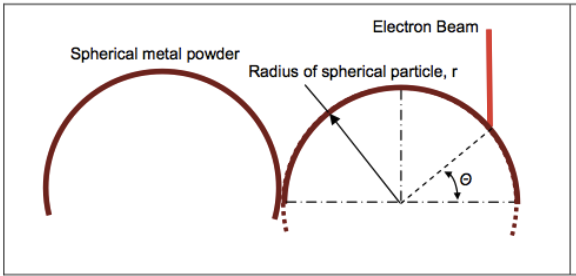
\includegraphics[scale=0.65]{Images/EBMparticles.png}
    }
    \qquad
    \subfloat[\label{fig:unsaccodiroba}]{
        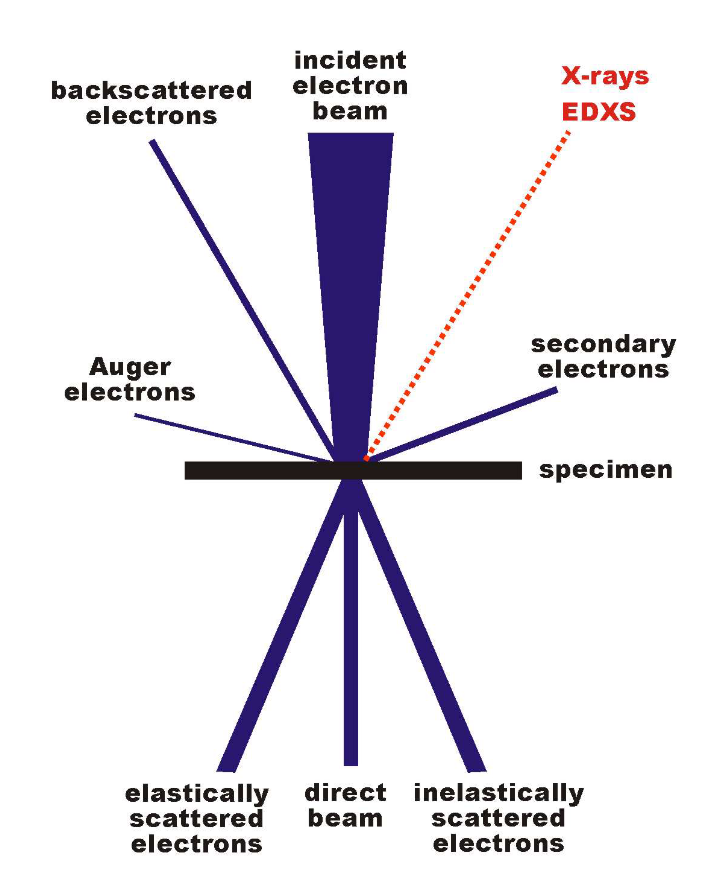
\includegraphics[scale=0.35]{Images/Screenshot 2023-08-21 at 11.42.27.png}
    }
    \caption[Laser interactions and laser intensity.]{Electron beam interaction with spherical powder particles (a) and Product from the interaction between an electron and a metal specimen (b) \cite{tushar_ramkrishna_mahale_electron_2009, krumeich_properties_2015}.}
\end{figure}
In Fig. \ref{fig:unsaccodiroba}, there is a schematic representation of the products resulting from the collision between an electron and a metal specimen.
% <<< End of Energy Matter Interactions

%%%%%
%%%%%

% Applications of PBF Metal Additive Manufacturing >>>
\section{Applications of PBF Metal Additive Manufacturing}
\label{sec:examplesPBF}
One of the primary advantages of PBF processes is the capability to produce finished objects unattainable with traditional manufacturing systems. In this section, we'll explore some examples of how this technology can completely disrupt the production processes of metal manufacturing. The nozzle in Fig \ref{fig:nozzle} is one of the more famous, successful, and documented examples of additive manufacturing for metal. General Electrics designed it in 2015. With AM, GE could produce the new nozzle in a single piece rather than 20 pieces welded together. They were able to reduce weight by 25\%, and it was five times more durable and 30\% more cost-efficient \cite{amy_kover_transformation_2018}. GE Aviation has set the goal of 32,000 nozzles per year in whole production \cite{milewski_additive_2017}, opening this manufacturing process to large scale distribution. In 2015, NASA designed the first 3D-printed rocket nozzle made of copper. Within the combustion chamber, the propellant burns at temperatures exceeding \SI{3000}{\kelvin}. Hydrogen at temperatures just above \SI{100}{\kelvin} flows through over 200 intricately designed cooling channels to prevent it from melting. The chamber's top rim integrates cooling inlets. Thanks to this new rocket nozzle, costs were reduced by 50\% and manufacturing times were reduced by ten times \cite{tracy_mcmahan_nasa_2015}, opening the path to a more affordable and lean space industry. Fig. \ref{fig:piston} shows Porsche's application of PBF processes in the automotive sector. The company managed to print pistons by PBF for the 911 GT2 RS engine. These new pistons have achieved a temperature on the piston's o-ring that is \SI{20}{\degreeCelsius} lower than usual. This leads to an additional \SI{23}{\kilo\watt} power available. However, before we see large-scale production, we'll have to wait until at least 2030 \cite{roberto_baldwin_porsches_2020} according to Porsche's press release. AM is also being employed in the medical field, for example, in dentistry. Custom-fitted designs are transforming the traditional ways of fabricating items like crowns and dental implants. Advanced high-precision 3D printers, such as EOS M 100 DMLS, can print devices from Cobalt Chrome SP2 alloy, a medical-grade approved material in the medical field \cite{milewski_additive_2017}. Products with small batch sizes, high precision, and significant value, like these dental devices, are increasingly manufactured using these new technologies. The advantages of AM include the swift creation of tailor-made items for immediate application, such as implants, or indirect uses like drill guides and fixtures, all based on the patient's medical characteristics for a perfect fit. Moreover, the surface finish or porous structures offer better support for bone growth. In Fig. \ref{fig:skul} there is an example of a titanium skull implant.
\begin{figure}
    \centering
    
    \subfloat[\label{fig:nozzle}]{
        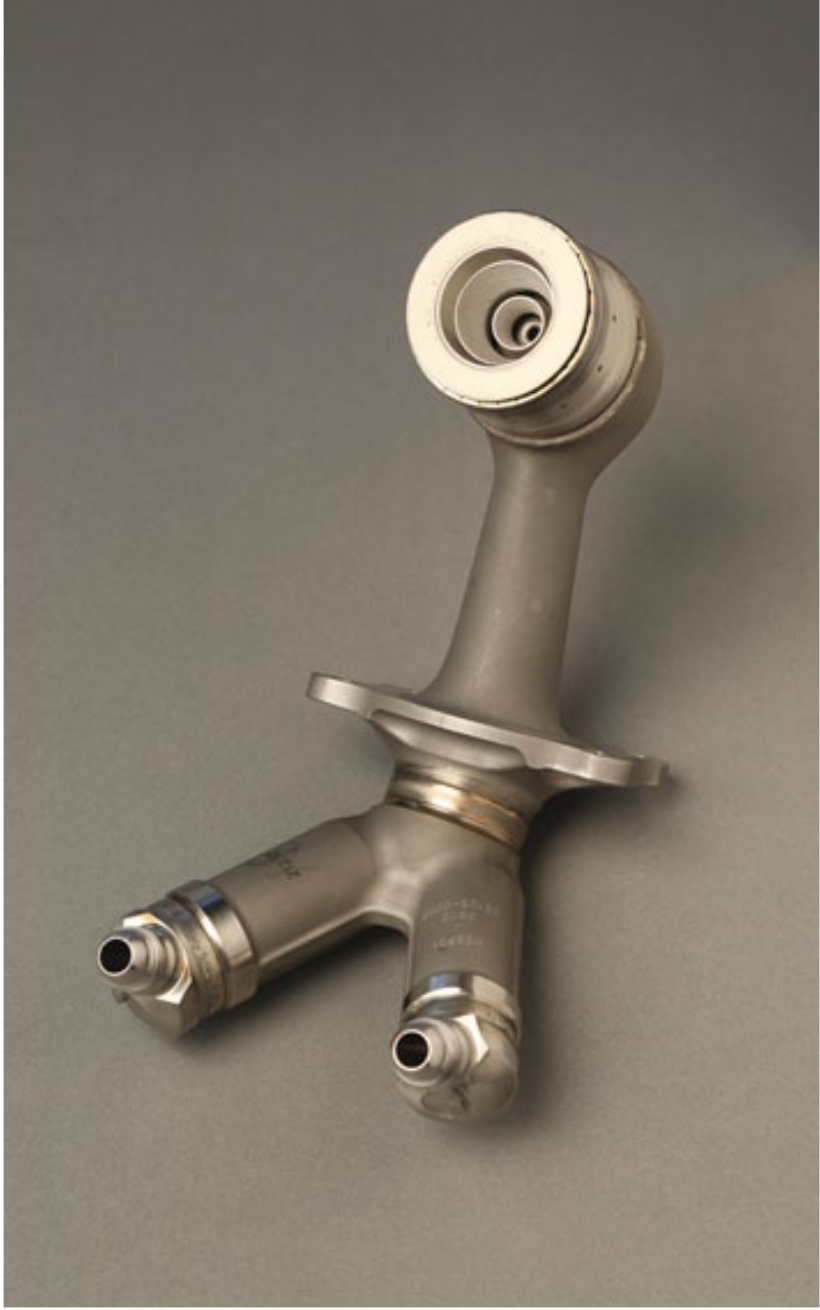
\includegraphics[scale=0.20]{Images/nozzle.png}
    }
    \qquad
     \subfloat[\label{fig:nozzlerocket}]{
        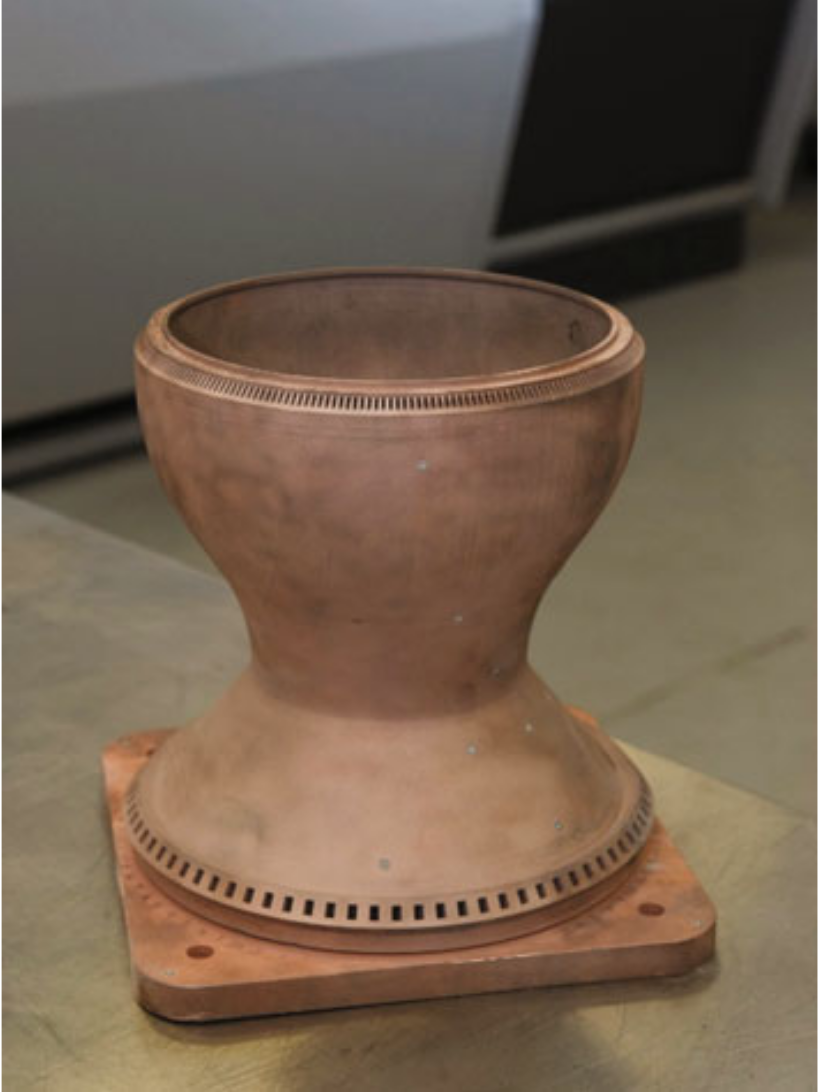
\includegraphics[scale=0.24]{Images/nozzlerocket.png}
    }
    \\
    \subfloat[\label{fig:piston}]{
        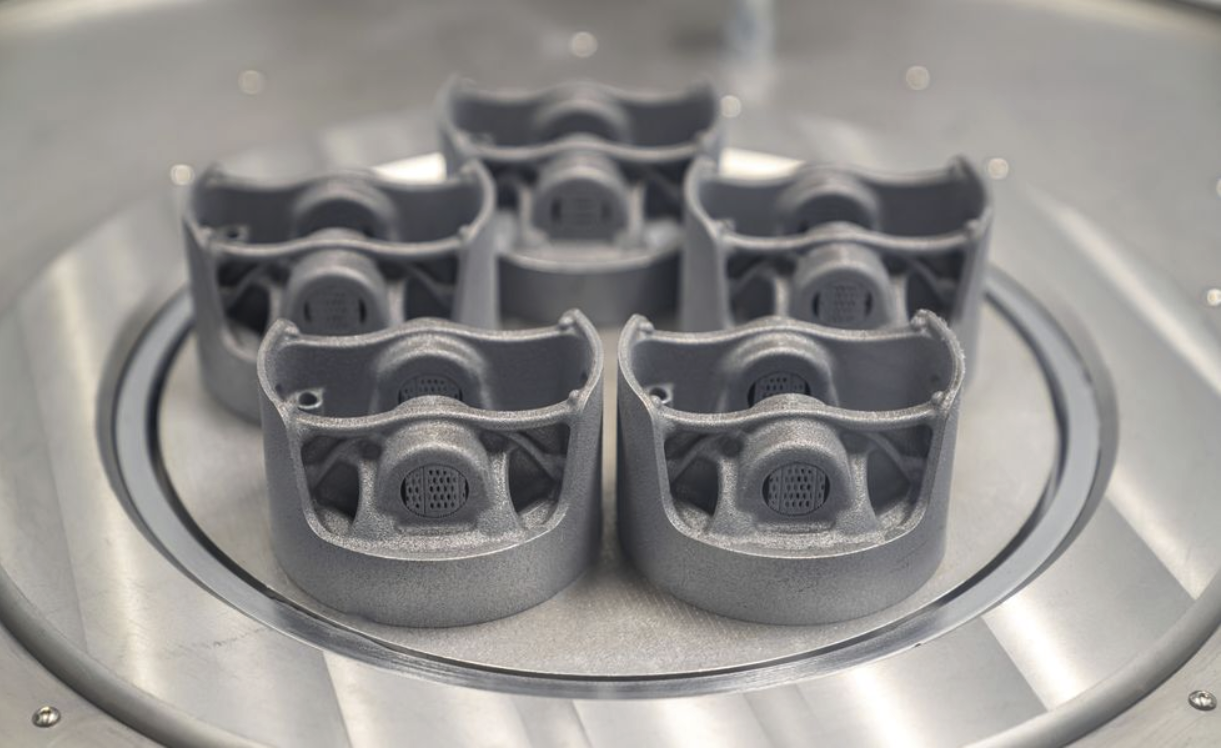
\includegraphics[scale=0.21]{Images/piston.png}
    }
    \qquad
    \subfloat[\label{fig:skul}]{
        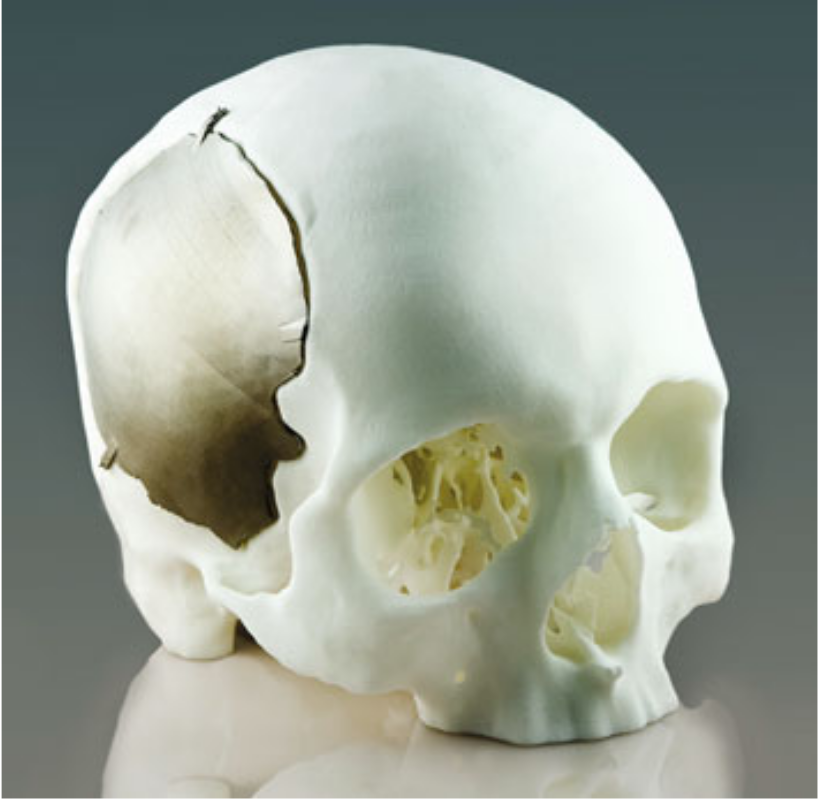
\includegraphics[scale=0.20]{Images/skull.png}
    }
    
    \caption[Examples of AM in metals.]{Examples of AM metal part: GE nozzle used in airplane turbines to mix fuel and air (a), a rocket nozzle in copper by NASA (b), Porsche engine pistons (c) and a titanium skull implant (d).}
    \label{fig:amexamples}
\end{figure}
\subsection{Lattice Structure and Cellular Material} \label{subsec:lattice}
A specific application of PBF processes is the printing of so-called lattice structures. According to ISO/ASTM 52900 \cite{organization_isoastm_2015}, \emph{lattice structure} are "three-dimensional geometric arrangement composed of connective links between vertices (points) creating a functional structure". Lattice structures are three-dimensional structures made up of different connected single elements called "cells" that can have different shapes designed to meet the desired mechanical features of the final object. These objects are distinguished by empty spaces within the structure. These structures can only be obtained thanks to layer-wise AM technologies. In recent years, the biomimicry technique has also spread in additive manufacturing. Biomimicry is a set of design techniques that allow us to take inspiration from nature to find solutions to engineering problems or to design functional components that can be used in engineering applications \cite{pathak_biomimicry_2019, du_plessis_beautiful_2019}. Over the past 3.8 billion years, nature has been able to find the most efficient way to develop functional solutions to evolutionary problems characterized by immovable constraints. Moreover, during the evolutionary process of species, nature has created nano, micro, and macro-structures that provide unique structural properties, adapting shape to function and using what is necessary to achieve the evolutionary goal. Indeed, one of life's principles explained in \citeauthor{baumeister_biomimicry_2011} (2011) states \textit{"Life integrates and optimizes these strategies to create conditions conducive to life"}. Therefore, it concerns creating new multi-functional structures with unique characteristics, optimizing materials, and reducing waste. Engineers have always been fascinated by cellular materials, evident from the first reference to the idea that structure could influence a material's functional characteristics and behavior, which Robert Hooke made in 1665 \cite{l_gibson_cellular_2010}. Only in recent years, thanks to the computational power of CAD softwares, it has been possible to experiment with the mechanical characteristics of 3D-printed lattice structures. Cellular materials are used mainly for their mechanical characteristics.
\begin{figure}
    \centering
    \subfloat[\label{fig:beehive}]{
        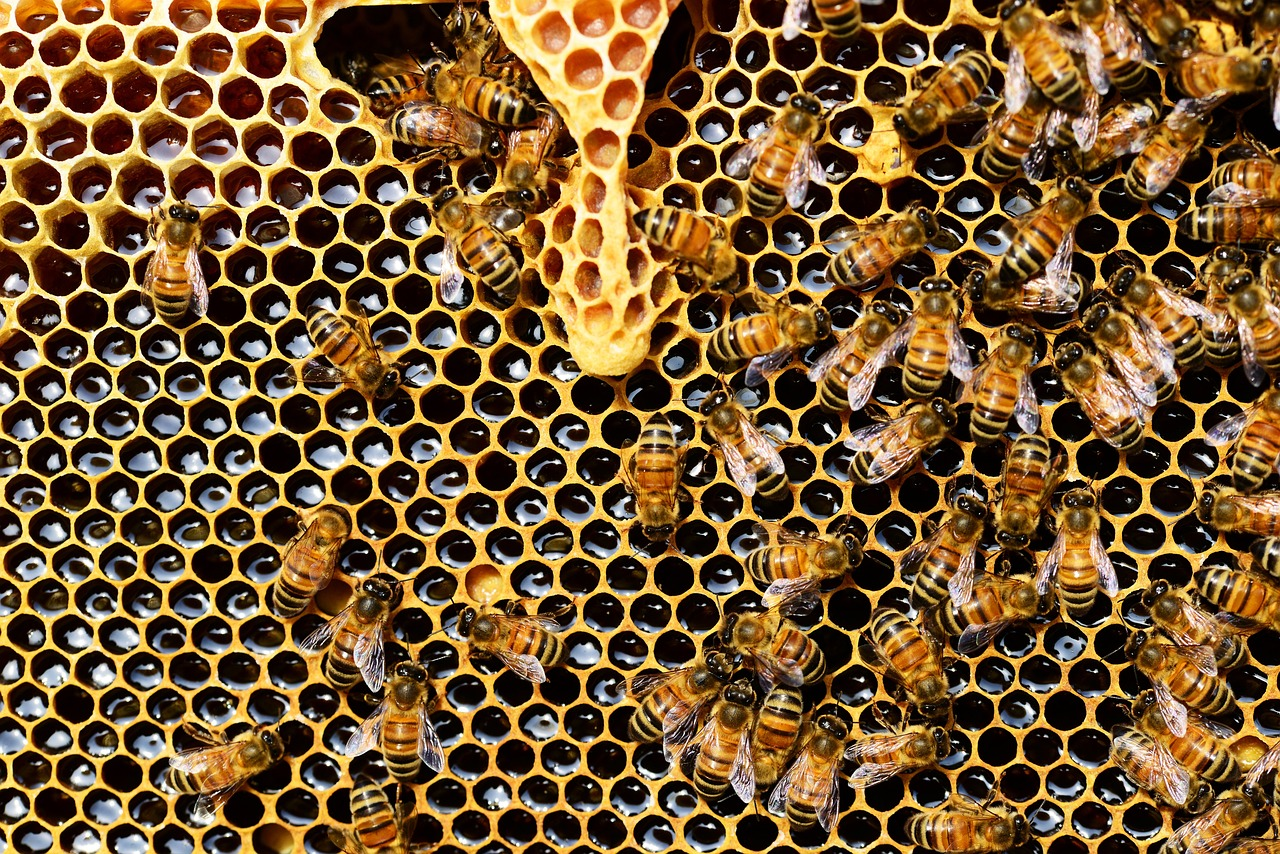
\includegraphics[scale=0.15]{Images/honey-bees-337695_1280.jpg}
    }
    \quad
    \subfloat[\label{fig:beelattice}]{
        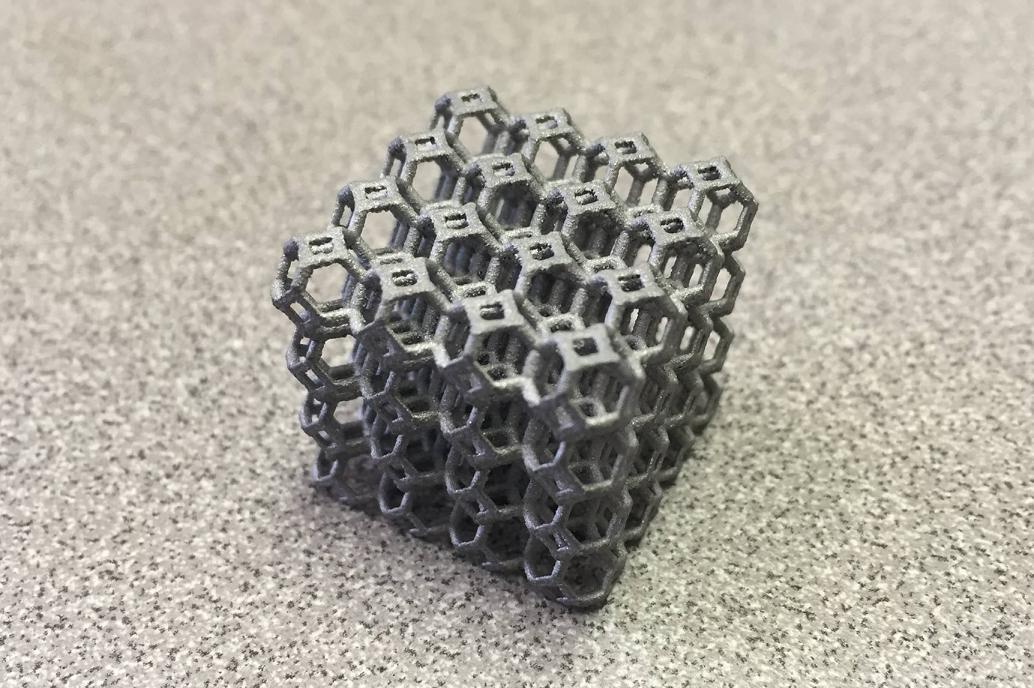
\includegraphics[scale=0.186]{Images/lattice1b.jpg}
    }
    \caption[Bio-inspiration design.]{An example of bio-inspiration design: from a beehive (a) to a lattice structure (b).}
    \label{fig:bioinsp}
\end{figure}
Just think that the aluminum cube in Fig. \ref{fig:beelattice} was printed using only \SI{3.9}{g} of material and can support a weight of \SI{408}{Kg}, which means it can withstand a stress 100,000 times its weight \cite{noauthor_3d_2014}. If we want to provide a more rigorous framework for classifying the applications of lattice structures in engineering, we can refer to the one proposed by \citeauthor{mcnulty_framework_2017}. According to this framework, cellular structures in nature exist primarily for three reasons:
\begin{itemize}
    \item \textbf{3D space-filling structures} may be the reason that most closely links the use of cellular structures in nature with AM, the need to confer strength to the structure while limiting its weight. Examples of this are the beehive, whose structure provides it with High specific stiffness under self-weight;
    \item \textbf{Surface structures}, enable surfaces to gain specific functional characteristics. For example, veining on the underside of the Amazon water lily leaf allows the leaf to gain excellent mechanical resistance, or the pomelo skin, with its open-cell structure, enables the fruit to resist impacts;
    \item \textbf{Cylindrical structures}: there are also examples of the use of cellular materials to confer particular characteristics to cylindrical structures (often hollow structures) that would otherwise be too fragile. For example, hedgehog quills have a particular internal structure that confers ovalization and buckling resistance to the quill.
\end{itemize}

\begin{figure}
    \centering
    \subfloat[\label{fig:heatexchanger}]{
        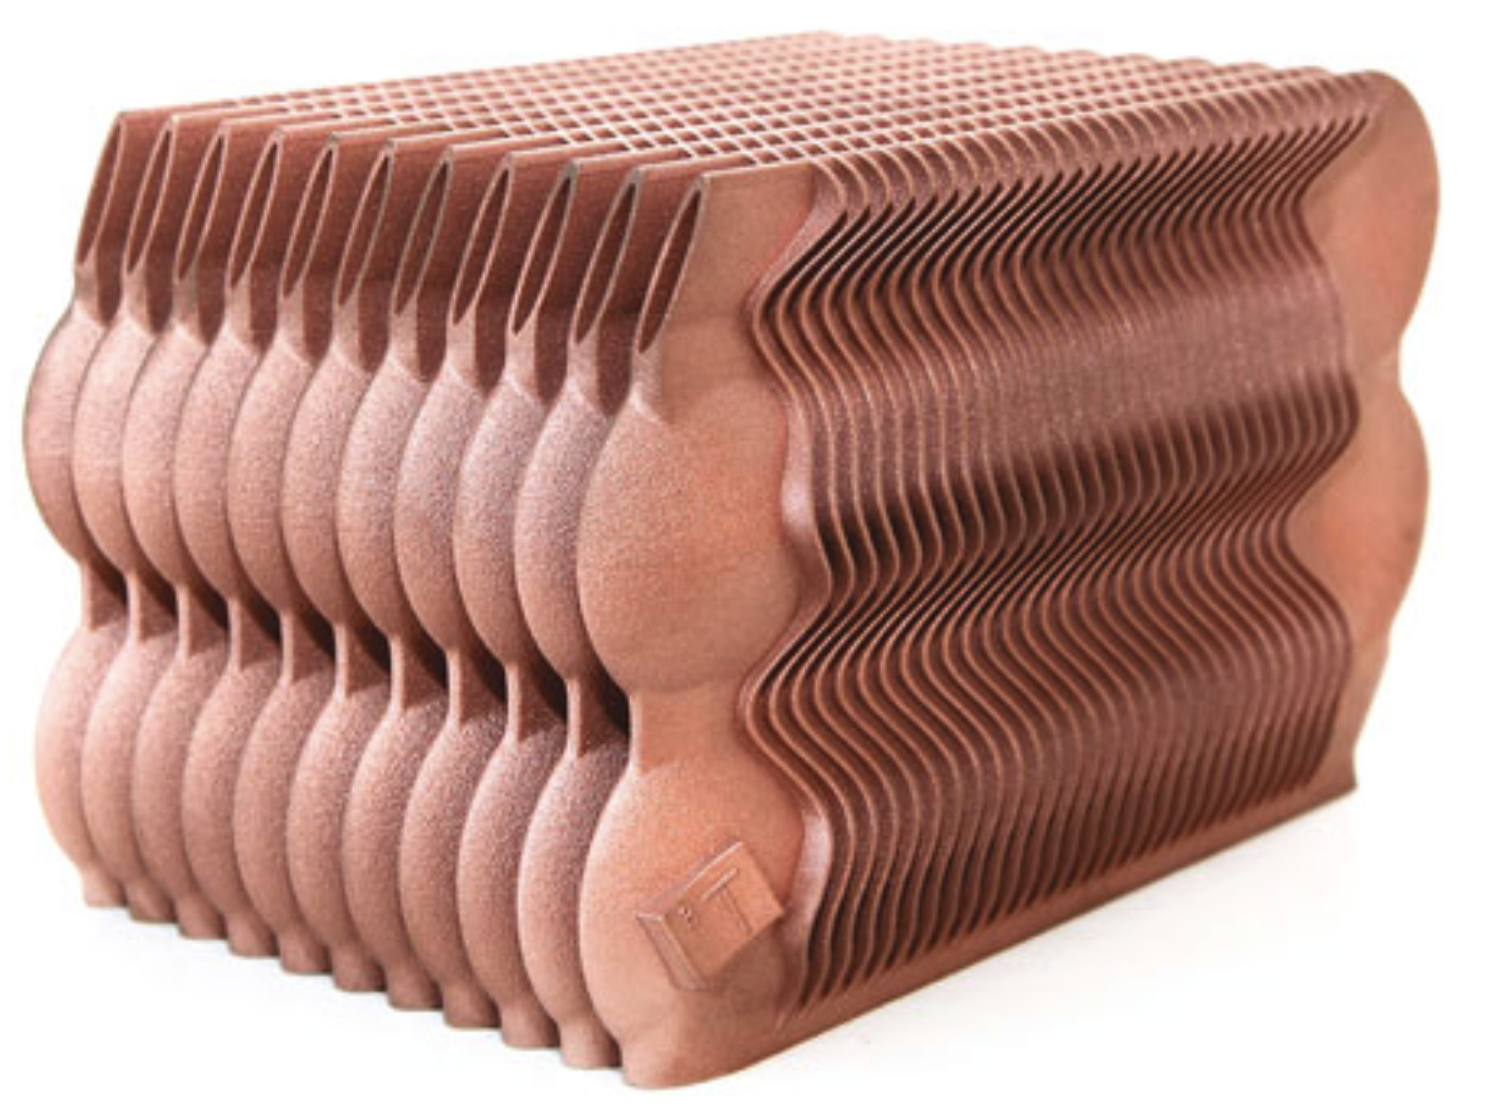
\includegraphics[scale=0.25]{Images/heatexchanger.png}
    }
    \qquad
    \subfloat[\label{fig:f1freno}]{
        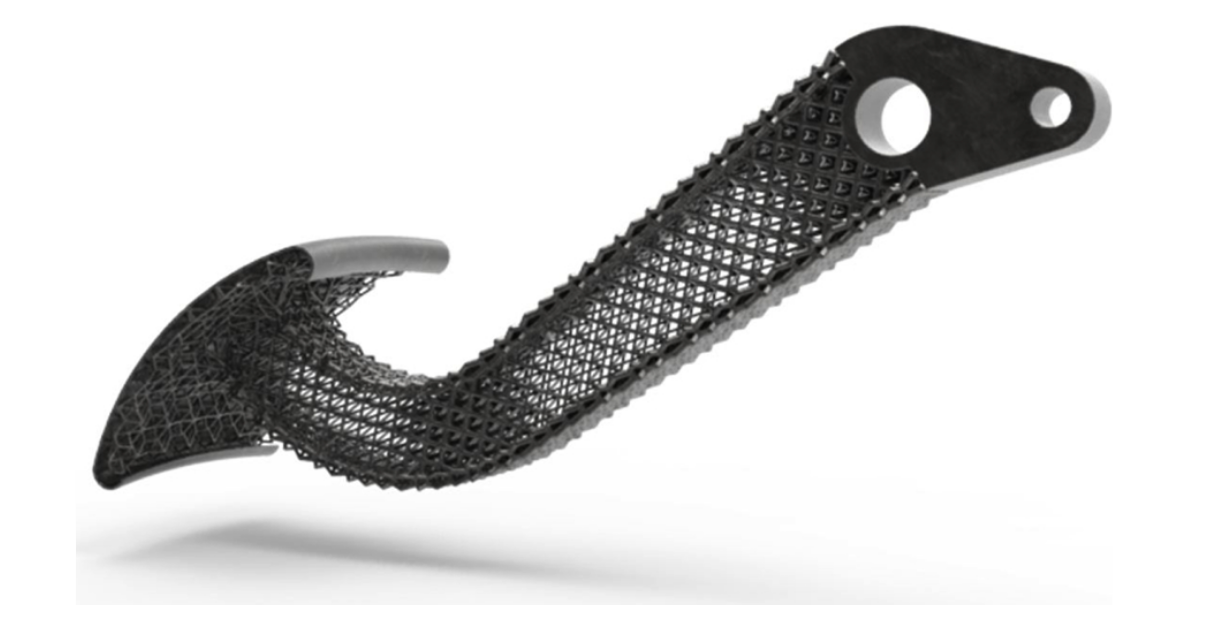
\includegraphics[scale=0.3]{Images/f1freno.png}
    }
    \caption[Lattice structure applications.]{Some lattice structure application: a complex heat exchanger (a) and brake pedal of F1 racing car (b) \cite{milewski_additive_2017, du_plessis_beautiful_2019}}.
\end{figure}

Lattice structures can be used for all these purposes, highlighting the incredible connection between nature and engineering. Lattice structures are versatile and can be effectively applied in various engineering fields to address multiple challenges. Specifically, they are commonly used in four main areas according to \citeauthor{bhate_classification_2019} (2019): 
\begin{itemize}
    \item \textbf{Structural engineering} for vibration control, strain isolation, and weight reduction purposes like in Fig. \ref{fig:f1freno};
    \item \textbf{Thermal engineering} for applications such as heat exchangers in Fig. \ref{fig:heatexchanger}, flame arresters, or heat shields;
    \item \textbf{Fluid dynamics engineering} which employs lattice structures as catalyst carriers or packaging;
    \item \textbf{Biomedical engineering}, where lattice structure can be leveraged for bone integration in prosthetic and cell growth
\end{itemize} 
Due to their unique properties, lattice structures are an attractive choice for engineers and designers seeking innovative solutions to complex problems across various industries, especially in the automotive, aerospace, energy and commodities, and medical industries.
% <<< End of Applications of PBF Metal Additive Manufacturing